\chapter{Numerical Methods}
\section{The Finite Element Method}
The theory presented in this section is partly inspired by the works of Langtangen in "Finite Element Method - INF5620 lecture notes" \cite{Lang2}  \\
Consider the Poisson-equation
\begin{align}
-\nabla^2 v = f & \quad \text{ in } \Omega \label{Poisson}\\
v = v_0 & \quad \text{ on } \partial \label{Poisson_D}\Omega_D \\
\pdi{v}{n} = g & \quad \text{ on } \partial \Omega_N \label{Poisson_N}
\end{align}
where $\Omega \in \mathbb{R}^d$ is a domain, $ v = v(x)$ is an unknown function and $f$ is a source function. The boundary, $\partial \Omega$ is divided into two parts. $\partial \Omega_D$ for the Dirichlet boundary condition, and $\partial \Omega_N$ for the Neumann condition. 
\\
\\
\subsection{Variational formulation}
\eqref{Poisson} is known as the strong form of the equation. To reformulate the problem and state a weak formulation we multiply the equation with a test function, $\phi \in \hat{V}$, where $\hat{V}$ is some function space, and integrate over the domain. Weak formulations are important in the sense that differential equations can be transformed into systems of linear equations. In the rest of this text the following notation is used for the inner product of two functions
\begin{align} (v,\phi)_{\Omega} = \int_{\Omega} v \, \phi \, \mathrm{d}x
\end{align}

By multiplying \eqref{Poisson} with a test function, $\phi$ and integrating over the domain, the weak form is obtained
\begin{align}
(\nabla^2 v + f, \phi)_\Omega = 0 & \quad \forall \, \phi \in\hat{V} \label{Projection}
\end{align}
We are now searching for a $v$ to satisfy the weak form instead of the strong. T
This equation should hold for all $\phi$ in the function space $\hat{V}$. The trial function does not necessarily have to lie in the same function space, in general $v \in V$. \\

 In this thesis we will use two Sobolov spaces (named after the Russian mathematician Sergei Sobolov) widely used in Finite Element computing. For these definitions to be valid, we assume that the functions $v$ are all \textbf{|locally integrable} and in the case of definition \eqref{H1}, has one \textbf{weak derivative}. For more details on weak derivatives and the generalized concept of Sobolev spaces and functional analysis, we refer to the textbook by Brenner and Scott \cite{Bren07}.   
\begin{definition}
Let $\Omega$ be an open subset of $\mathbb{R}$ with a piecewise smooth boundary. We then define the $L^2$-norm as follows\\ \begin{center}
$||v||_{L^2(\Omega)} = (\int_\Omega v^2 \mathrm{d}x)^{\frac{1}{2}}$
\end{center}
The corresponding $L^2$-space is defined via
\begin{center}
$L^2(\Omega) = \{ v:\Omega \rightarrow \mathbb{R} | \int_\Omega v^2 \mathrm{d}x < \infty \}$
\end{center}
\label{|l2}
\end{definition}
\begin{definition}
Let $\Omega$ be an open subset of $\mathbb{R}$ with a piecewise smooth boundary. We then define the $H^1$-norm as follows\\ \begin{center}
$||v||_{H^1(\Omega)} = (\int_\Omega [v^2 + (\nabla v)^2]\mathrm{d}x)^{\frac{1}{2}}$
\end{center}
The corresponding $H^1$-space is defined via
\begin{center} $H^1(\Omega) = \{ v:\Omega \rightarrow \mathbb{R} | \int_\Omega [v^2 + (\nabla v)^2] \mathrm{d}x < \infty \}$
\end{center}
\label{H1}
\end{definition}
In other words, using functions from these spaces, we can have some assurance that the integrals involved in the variational form are bounded. 
By the divergence theorem, a generalized concept of integration by parts we can state the variational problem as follows: find $v \in V$ such that \\ \\
\begin{align}
(\nabla v, \nabla \phi)_\Omega = (f,\phi)_\Omega + (g, \phi)_{\partial \Omega_N}& \quad \forall \, \phi \in \hat{V} \label{Weak_form}
\end{align}
\\
Where we have used that $\pdi{v}{n} = g$ on $\partial \Omega_N$. \eqref{Weak_form} is known as the variational formulation of the Poisson problem.  The left hand side is known as the bilinear form while the right hand side is the linear form. In generic form the equation can be written
\begin{align}
a(v,\phi) = L(\phi) \label{Bilinear}
\end{align}
The first derivative of $v$ appears in the variational form. A common choice is then
\begin{align}
 V := \{ v \in H^1(\Omega) : v = v_0 \text{ on } \partial \Omega_D \} \\
 \hat{V} := \{ v \in H^1(\Omega) : v = 0 \text{ on } \partial \Omega_D \}
\end{align}
In other words, the trial and test functions are in the same function space, except on the boundary.



\subsection{Finite elements} \label{FinEle}
The next step is to approximate $v$ with a sum of basisfunctions in the finite-dimensional function space, $V = \text{span}\{\phi_0, \phi_1, ..., \phi_N \}$. Here, $\phi_i$ represents the basis functions and we search for a solution $v_h \in V$ such that $v_h$ can be written as a linear combination of the basis functions. 
The first step in the finite element method consists of dividing the domain into smaller parts
\begin{align*}
\Omega = \Omega_0 \cup \Omega_1 \cup ... \cup \Omega_{N_e}
\end{align*}
where $N_e$ is the number of elements. Each element have a number of nodes within them depending on what type of basis functions to be used. Let's first consider the continuous Galerkin basis functions, in a one-dimensional domain. There is exactly one basisfunction for each node located at $x_i$. These basis functions have the property that
\begin{align*}
\phi_i(x_j) = \begin{cases}
				1 \quad \text{ for } i=j \\
				0 \quad \text{ for } i\neq j
		 		\end{cases}
\end{align*}
\begin{figure}[!ht]
  \begin{center}
    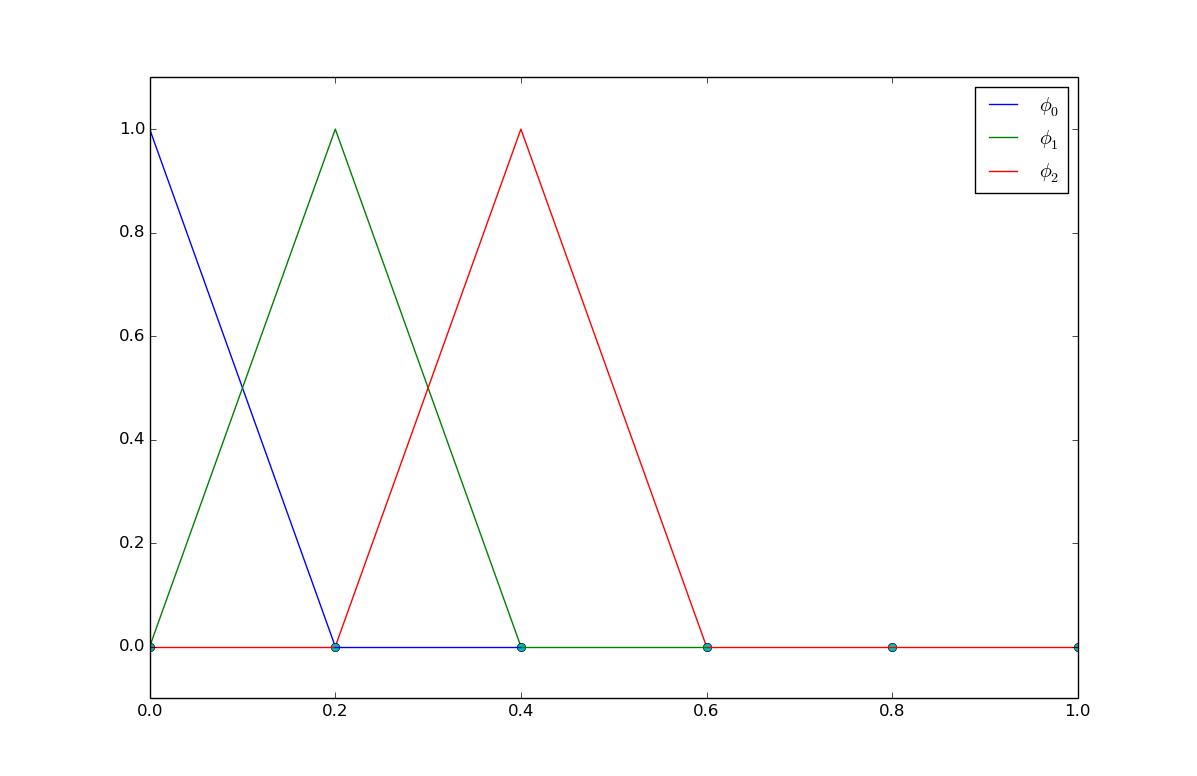
\includegraphics[scale=0.4]{figures/hats.png}
  \end{center}
	\caption{The three first linear basis functions on the unit interval divided uniformly into 5 elements, $\Omega_0 = [0,0.2], \Omega_1 = [0.2,0.4]$ and so on. In the case of Dirichlet Boundary conditions at $x=0$, $\phi_0$ will not be included in the funtcion space}
	\label{fig:Hats}
\end{figure}
\\
That is, the basis functions $\phi_i$ are zero on all nodes except at node $i$. Each basis function is constructed by taking the Lagrange-polynomial which is 1 at the given node and 0 on the neighboring nodes. Note that the basis functions are two Lagrange-polynomials "pieced together" at the node where it's value is 1. For the rest of the domain the basis functions are defined to be 0. \\ \\

Now, let's return to the original problem \eqref{Poisson}-\eqref{Poisson_N} in scalar form. We start by approximating $v$ as a linear combination of all the basis functions. 
\begin{align}
v_h = \sum_{i=0}^N c_i \phi_i \label{u_hsum}
\end{align}
The definitions of $v_h$ and $V$ now give rise to a linear system. Using the Einstein summation convention, $x_i\,y_i = \sum_0^N x_i y_i $, the discretized version of \eqref{Weak_form} is now written 
\begin{align}
-c_i(\nabla \phi_i, \nabla \phi_j)_\Omega = (f,\phi_j)_\Omega - (g, \phi_j)_{\partial \Omega_N} \label{|linear_system}
\end{align}
\\
\\

In the case of Dirichlet boundary conditions all test functions $\phi_j$ will take the value 0 on $\partial \Omega_D$ and the linear system will be adjusted to take these boundary conditions into account. \\
The system can be written in matrix form, and in the end the problem consists of solving the linear system
\begin{align} A_{i,j}c_i = b_j \label{Matrix_1} \end{align}
\\
\\
\subsection{Implementation in FEniCS}
When the variational form has been carried out, implementation in FEniCS is relatively simple. The programs in this study are written in the Python programming language. When programming with Python, we first need to import dolfin to access the DOLFIN library, containing classes convinient and efficient for finite element computing. In Python the full library can be imported as simple as 
\begin{verbatim}
from dolfin import *
\end{verbatim}
Now, let's focus our attention on solving the following problem:
\begin{align}
\nabla^2v = 20x \,\,\,\,\, \text{ in } \Omega \\
v(0,y) = 0, \,\,\,\, v(1,y) = 1 \\
\pdi{v(x,0)}{n} = \pdi{v(x,1)}{n} = 0
\end{align}
Where $\Omega$ is the unit square, $\Omega = [0,1] \times [0,1]$ \\
\\
First of all we need to define the computational mesh.
\begin{cverbatim}
mesh = UnitSquareMesh(10,10)
\end{cverbatim}
The class UnitSquareMesh initializes a mesh with triangular cells. The mesh consists of n$\times$m squares depending on the arguments, $n$ and $m$, sent into the constructor. Each of these squares are divided on the diagonal to form two triangles, and these triangles are the computational cells. In this case we get the unit square divided into 10$\times$10 smaller squares and thus the total number of triangles, or cells, will be 200. \\
The next thing to do is to define an appropriate function space for the test functions. The solution will be a linear combination of these functions and will be in (almost) the same function space. 
\begin{cverbatim}
V = FunctionSpace(mesh,'CG',1)
\end{cverbatim}
The function space needs a domain, type of element, and the degree of the element. In this case we use Continuous Galerkin elements ('CG') with degree 1. These basis functions are visualized in Figure \ref{fig:Hats}
\\ We can then define our test- and trial functions $v$ and $\phi$
\begin{cverbatim}
v = TrialFunction(V)
phi = TestFunction(V)
\end{cverbatim}
Note that the test- and trial function seem to be in the exact same function space. This is the case except when imposing Dirichlet boundary conditions. 
The functions $f$, $v_0$ and $g$ can be defined by using the 'Constant' or 'Expression' classes. We set $f = 20x$ and use Dirichlet boundary conditions, $v(0,y) = 0$, $v(1,y) = 1$ and Neumann conditions $\pdi{v(x,0)}{n} = \pdi{v(x,1)}{n} = 0$. The homogenuous Neumann condition is simple in the finite element method as the terms appearing after integration by parts can be dropped. If this is not the case, we can insert $g$ for $\pdi{u}{n}$ on the boundary integral appearing in the variational form. When the Neumann conditions are incorporated this way we say that the boundary conditions are weakly imposed. Functions (or classes) describing the boundaries must also be defined:
\begin{cverbatim}
f = Expression('20*x[0]')
def boundary0(x,on_bnd):
	return on_bnd and near(x[0],0.0)
def boundary1(x,on_bnd):
	return on_bnd and near(x[0],1.0)

bc0 = DirichletBC(V,0.0,boundary0)
bc1 = DirichletBC(V,1.0,boundary1)
bcs = [bc0,bc1]
\end{cverbatim}
Note that 'x[0]' means first dimension in space, 'x[1]' means second dimension and so on. The Dirichlet conditions are put in a list. Next, the variational form is defined, and when solving for a function v, the boundary conditions are added to the "magic" solve function. 
\begin{cverbatim}
F = inner(grad(v),grad(phi))*dx - inner(f,phi)*dx
v = Function(V)
solve(lhs(F)==rhs(F),v,bcs)
plot(v)
\end{cverbatim}
The functions lhs and rhs separates the form F into the left hand side, equivalent to the bilinear form and to the right hand side, equivalent to the linear form. Specifying the full form F is simple and convenient when the equations are short and simple. If we want to relate the code to the mathematics as written in \eqref{Bilinear} we can, define these forms manually. 
\begin{cverbatim}
a = inner(grad(v),grad(phi))*dx
L = inner(f,phi)*dx
v = Function(V)
solve(a==L,v,bcs)
\end{cverbatim}
\begin{figure}[!h]
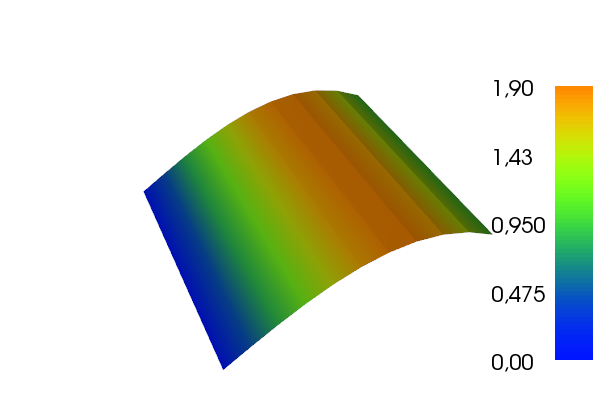
\includegraphics[scale=0.5]{figures/poisson_f_20x}
\caption{Plot of the computed solution}
\end{figure}
The plot in the figure is slightly rotated. The solution is independent of y-position, as expected. 


\section{A bencmark FSI-problem}
Within CFD, a benchmark is a configuration or a test case which should help test and compare different numerical methods and code implementations. A classical Fluid Dynamics problem regarding flow around a circular cylinder has been under vast research the last 50 years, working as a test case for both laminar and turbulent flows. One of the most cited benchmark proposals for this case is the problem described by Michael Schafer et. al in 1996 \cite{Scha96}. The research group still focus on these kinds of problems and one of the co-authors of the 1996 paper, Stefan Turek, together with Jaroslav Hron has proposed a similar benchmark for FSI solvers, consisting of the exact same domain and rigid cylinder, but now with an elastic flag attached to it \cite{Ture06}. 
\\ The first results presented will contain a validation of the present FSI-solver implemented in FEniCS compared to the results of Turek and Hron in their benchmark proposal. 
\begin{figure}
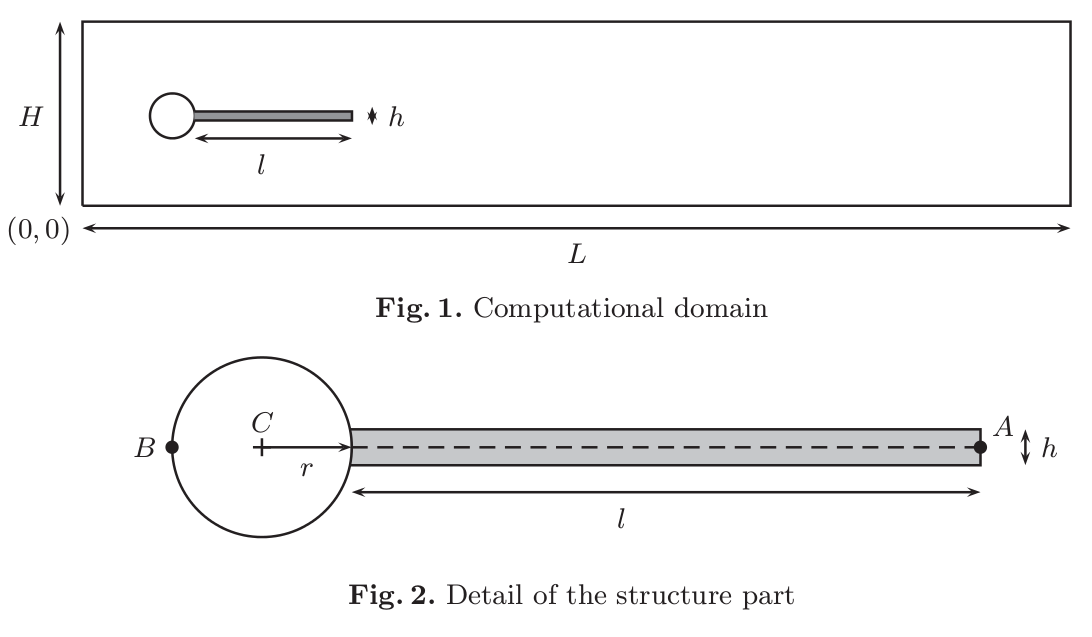
\includegraphics[scale=0.3]{figures/Hron_Turek_geometry}
\caption{The Domain as published in \cite{Ture06}}
\label{fig:Geometry}
\end{figure}
\\
A proper validation of a FSI solver requires separate verification of the fluid and structural parts as well as coupled tests. In the present study we solve the system of equations with a \textit{monolithic} approach, i.e. full coupling between the fluid and solid. The alternative would be a \textit{partitioned} approach, where the fluid and solid equations are solved separately. For instance, one can solve the fluid equations independently and then proceed by solving the solid equation with prescribed stress on the interface computed from the fluid solution. Iteration back and forth would be needed until convergence. \\
The fully coupled monolithic scheme is usually preferred with respect to accuracy and stability. Also, when the systems are strongly coupled in nature, i.e. the solid movement is affected by the fluid movement and vice versa, a monolithic scheme would be advantageous. The partitioned approach, on the other hand, can benefit from numeruous previous studies where efficiency and stability for various solution techniques have been investigated. See e.g. \cite{Tang14} for a short review. In addition, solving many smaller matrix systems will be way faster than solving one large system with the same number of unknowns.
\\
\\
\subsection{Domain, Initial- and boundary conditions}
The origin is set at the bottom left corner. We also set:
\\ - The channel height, H = 0.41
\\ - The channel length, L = 2.5
\\ - The circle center C = (0.2,0.2)
\\ - The right bottom corner of the elastic structure has position (0.6,0.19) 
\\ - The elastic structure has length, l=0.35 and heigth h=0.02
\\
\\
- At the left boundary, the inlet, of the channel, we set a prescribed parabolic velocity profile
\begin{align}
\mathbf{v}_{\text{in}}(0,y) = 1.5\bar{v_0}\frac{y(H-y)}{(\frac{H}{2})^2}
\end{align}
- In the case of unsteady flow a smooth increase in time is used:
\begin{align}
 \mathbf{v}_{\text{in}}(t,0,y)= \begin{cases}
				\mathbf{v}_{\text{in}}(0,y)\frac{1-\cos(\frac{\pi}{2}t)}{2} & \quad \text{ if } t<2.0 \\
				\mathbf{v}_{\text{in}}(0,y) & \quad  \text{ otherwise }
		 		\end{cases}
\end{align}
\\
- On the outlet, the condition $\sigma \cdot \mathbf{n} = 0$) is applied
- On rigid walls the no-slip condition is used
- On the interface, $\Gamma^t$, the previously described coupling conditions are applied:
\begin{align}
\begin{rcases}
\sigma_f \cdot \mathbf{n} & =  \sigma_s \cdot \mathbf{n} \\
\mathbf{v}_f & = \mathbf{v}_s
\end{rcases}
\text{ on } \Gamma^t
\end{align}
In addition to the interface, $\Gamma^t$, it may be convenient to define the fluid boundary, $\partial \Omega_f^t$ consisting of the outer rectangle and the part of the circle in contact with the fluid, and the solid boundary, $\partial \Omega_s^t$ consisting of the circle in contact with the solid.
\subsection{CFD tests}
For the CFD tests we perform tests treating the flag as a rigid object. This can be done by changing the structural parameters, or simply by adjust the mesh to include the fluid domain only. In this validation we choose the latter. We show convergence with Mesh, where mesh 0 is the coarsest version. The \textbf{Ref.} are the reference values as given in the original benchmark paper. 

\begin{table}[!ht]
\begin{center}
  \begin{tabular}{|l | l | l | l|} \hline
	Parameter & CFD1 & CFD2 & CFD3 \\ \hline
    $\rho_f\, [10^3\frac{\text{kg}}{\text{m}^3}]$  & 1 & 1 & 1 \\   \hline
    $\nu_f\, [10^{-3}\frac{\text{m}^2}{\text{s}}]$ & 1 & 1 & 1 \\ \hline
    $\bar{v_0}$ & 0.2 & 1 & 2   \\ \hline \hline
    $\text{Re} = \frac{Ud}{\nu_f}$ & 20 & 100 & 200 \\ \hline 
    \hline
  \end{tabular}
  \caption{Parameters for the CFD test cases}
\end{center}
\end{table}
\begin{table}[!ht]
\begin{center}
  \begin{tabular}{|l | l | l | l|} \hline
	cells & dofs & Drag & Lift \\ \hline
    1334  & 6443 & 13.9344 & 1.0980  \\   \hline
    5336 & 24892 & 14.1165 & 1.0836 \\ \hline
    21344 & 97808 & 14.1865 & 1.0944  \\ \hline \hline
    \textbf{Ref.}  & & \textbf{14.29} & \textbf{1.119} \\ \hline 
    \hline
  \end{tabular}
\end{center}
\caption{Results for CFD1}
\end{table}

\begin{table}[!ht]
\begin{center}
  \begin{tabular}{|l | l | l | l|} \hline
	cells & dofs & Drag & Lift \\ \hline
    1334  & 6443 & 130.092948352 & 10.9117261826 \\   \hline
    5336 & 24892& 134.43022177 & 10.473965217 \\ \hline
    21344 & 97808& 135.777285175 & 10.7118857057 \\ \hline \hline
    \textbf{Ref.}  & & \textbf{136.7} & \textbf{10.53} \\ \hline 
    \hline
  \end{tabular}
\end{center}
\caption{Results for CFD2}
\end{table}
\begin{table}[!ht]
\begin{center}
	\begin{tabular}{|l | l | l | l|} \hline
	cells & dofs & Drag & Lift \\ \hline
    1334  & 6443& 391.305 $\pm$ 2.039 & -28.536 $\pm$ 200.149\\   \hline
    5336 & 24892  & 428.769 $\pm$ 5.735 & -18.001 $\pm$ 429.410 \\ \hline
    21344 & 97808& 1 & 2   \\ \hline \hline
    \hline
  \end{tabular}
  \begin{tabular}{|l | l | l | l|} \hline
	cells & dofs & Drag & Lift \\ \hline
    755  & 6443  &  391.401 $\pm$ 2.460  & -22.652 $\pm$ 232.090\\   \hline
    5336 & 24892 & 428.787 $\pm$ 5.773 & -14.575 $\pm$ 441.152 \\ \hline
    21344 & 97808& 1 & 2   \\ \hline \hline
    \textbf{Ref.}  & & \textbf{439.45 $\pm$ 5.6183} & \textbf{-11.893 $\pm$ 437.81} \\ \hline 
    \hline
  \end{tabular}
\end{center}
\caption{Results for CFD3 for $\Delta t = 0.0005$ and $\Delta t = 0.0001$} 
\end{table}

\subsection{CSM tests}
The structural tests are performmed by adding the gravitational force to the structural part only. The CSM3 test is computed as a time-dependent case, starting from the initial position while CSM1 and CSM2 are Steady State (SS) solutions. For CSM3, the total energy is not conserved as the Backward Euler scheme used to discretize in time sligthly recudes the amplitude for oscillating solutions. For this reason, a third parameter of interest is included in the results, namely the reduction of amplitude from one cycle to the next. From the reference results it appears that the flag bounces above the initial position in steady state, meaning that some energy must have been added due to their choice of scheme. This is also clear when closely examining the attached plots. This was not further discussed, and no time-dependent amplitude was reported. The temporal discretization in the original benchmark proposal was done by the Cranck-Nicholson scheme, which in general have better conservation properties than the Backward-Euler scheme but is known to be less stable \cite{Hron06}
\begin{table}[!ht]
\begin{center}
  \begin{tabular}{|l | l | l | l|} \hline
	Parameter & CSM1 & CSM2 & CSM3 \\ \hline
    $\rho_s\, [10^3\frac{\text{kg}}{\text{m}^3}]$  & 1 & 1 & 1 \\   \hline
    $\nu_s $ & 0.4 & 0.4 & 0.4 \\ \hline
    $\mu_s \,[10^{6}\frac{\text{m}^2}{\text{s}}]$ & 0.5 & 2 & 0.5   \\ \hline
    $g \, [\frac{\text{m}^2}{s}]$ & 2 & 2 & 2 \\ \hline
    \hline
  \end{tabular}
\end{center}
\caption{Parameters for the CSM test cases}
\end{table}

\begin{table}[!h]
\begin{center}
  \begin{tabular}{|l | l | l | l|} \hline
	cells & dofs & $U_x$ of A $[10^{-3}]$ & $U_y$ of A $[10^{-3}]$\\ \hline
	738  & 4596  & -12.410569 & -60.599246 \\   \hline
	2952 & 17305 & -12.419505 & -60.622920 \\ \hline
	11808 & 67077 & -12.422290 & -60.630433   \\ \hline \hline
    \textbf{Ref.}  & & \textbf{-7.187} & \textbf{-66.10} \\ \hline 
    \hline
  \end{tabular}
\end{center}
\caption{Results for CSM1}
\end{table}

\begin{table}[!h]
\begin{center}
  \begin{tabular}{|l | l | l | l|} \hline
	cells & dofs & $U_x$ of A $[10^{-3}]$ & $U_y$ of A $[10^{-3}]$\\ \hline
   738  & 4596  & -0.92479395 & -16.853778 \\   \hline
   2952 & 17305 & -0.92558954 & -16.861757 \\ \hline
   11808 & 67077 & -0.92583356 & -16.864252   \\ \hline \hline
    \textbf{Ref.}  & & \textbf{-0.4690} & \textbf{-16.97} \\ \hline 
    \hline
  \end{tabular}
\end{center}
\caption{Results for CSM2}
\end{table}

\begin{table}[!h]
\begin{center}
  \begin{tabular}{|l | l | l | l| l|} \hline
	cells & dofs & $U_x$ of A $[10^{-3}]$ & $U_y$ of A $[10^{-3}]$ & Amp reduction y (\%) \\ \hline
    738  & 4596 & -44.175 $\pm$ 44.007 & -72.712 $\pm$ 65.281 & 5.4  \\   \hline
    2952 & 17305 & -44.176 $\pm$ 44.001 & -72.720 $\pm$ 65.281 & 5.4 \\ \hline
    11808 & 67077 & -44.177 $\pm$ 44.001 & -72.720 $\pm$ 65.281 & 5.4  \\ \hline \hline
    \textbf{Ref.}  & & -\textbf{14.305} $\pm$ \textbf{14.305} & -\textbf{63.607} $\pm$ \textbf{65.160} \\ \hline 
    \hline
  \end{tabular}
\end{center}
\end{table}


\begin{table}[!h]
\begin{center}
  \begin{tabular}{|l | l | l | l| l|} \hline
	cells & dofs & $U_x$ of A $[10^{-3}]$ & $U_y$ of A $[10^{-3}]$ & Amp reduction y (\%) \\ \hline
    738  & 4596 & -44.631 $\pm$ 44.628 & -69.702 $\pm$ 69.290 & 0.3  \\   \hline
    2952 & 17305& -44.633 $\pm$ 44.629 & -69.701 $\pm$ 69.289 & 0.3 \\ \hline
    11808 & 67077& -44.094 $\pm$ 44.091 & -69.703 $\pm$ 69.289 & 0.3  \\ \hline \hline
    \textbf{Ref.}  & & -\textbf{14.305} $\pm$ \textbf{14.305} & -\textbf{63.607} $\pm$ \textbf{65.160} \\ \hline 
    \hline
  \end{tabular}
\end{center}
\caption{Results for CSM3, $\Delta t= 0.01, 0.001$}
\end{table}


\begin{figure}[!ht]
\begin{subfigure}[b]{0.5\linewidth}
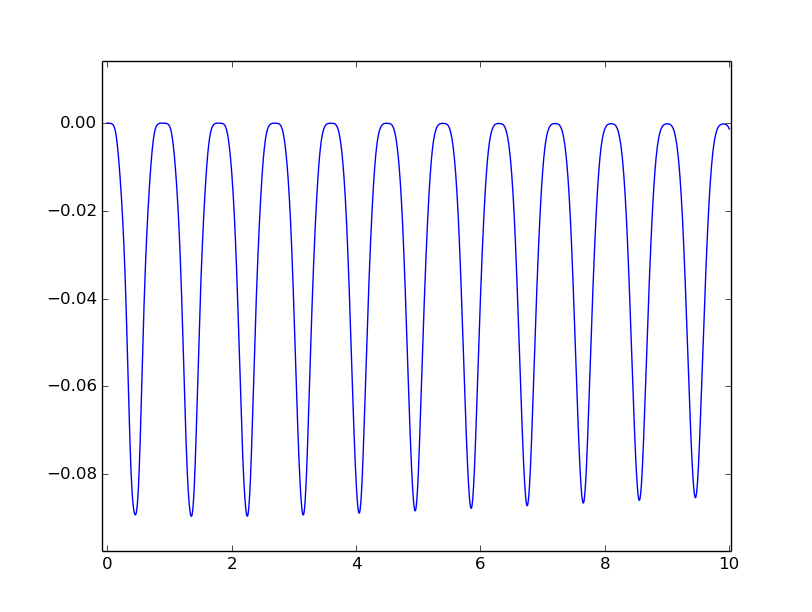
\includegraphics[width=\linewidth]{figures/CSM3/CSM3_Full_x}\caption{displacement x vs time}
\end{subfigure}
\begin{subfigure}[b]{0.5\linewidth}
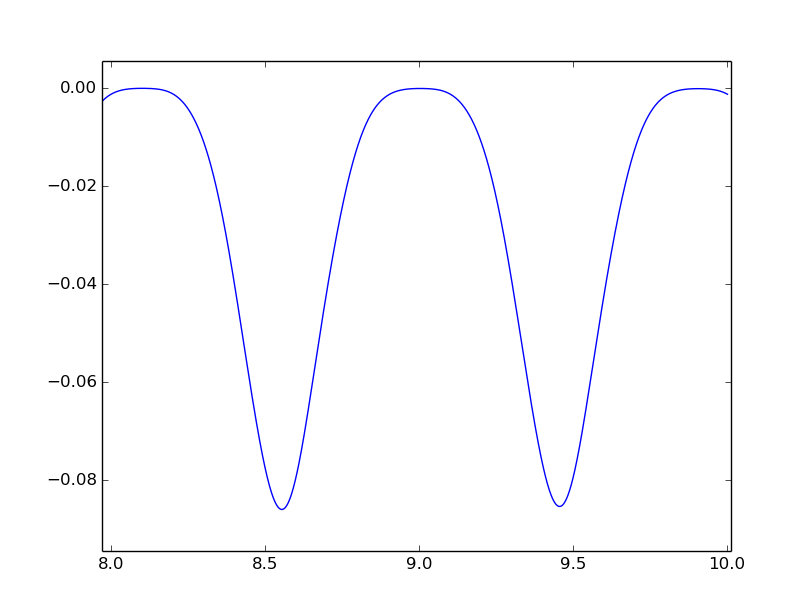
\includegraphics[width=\linewidth]{figures/CSM3/CSM3_2_x}\caption{displacement x vs time}
\end{subfigure}
\begin{subfigure}[b]{0.5\linewidth}
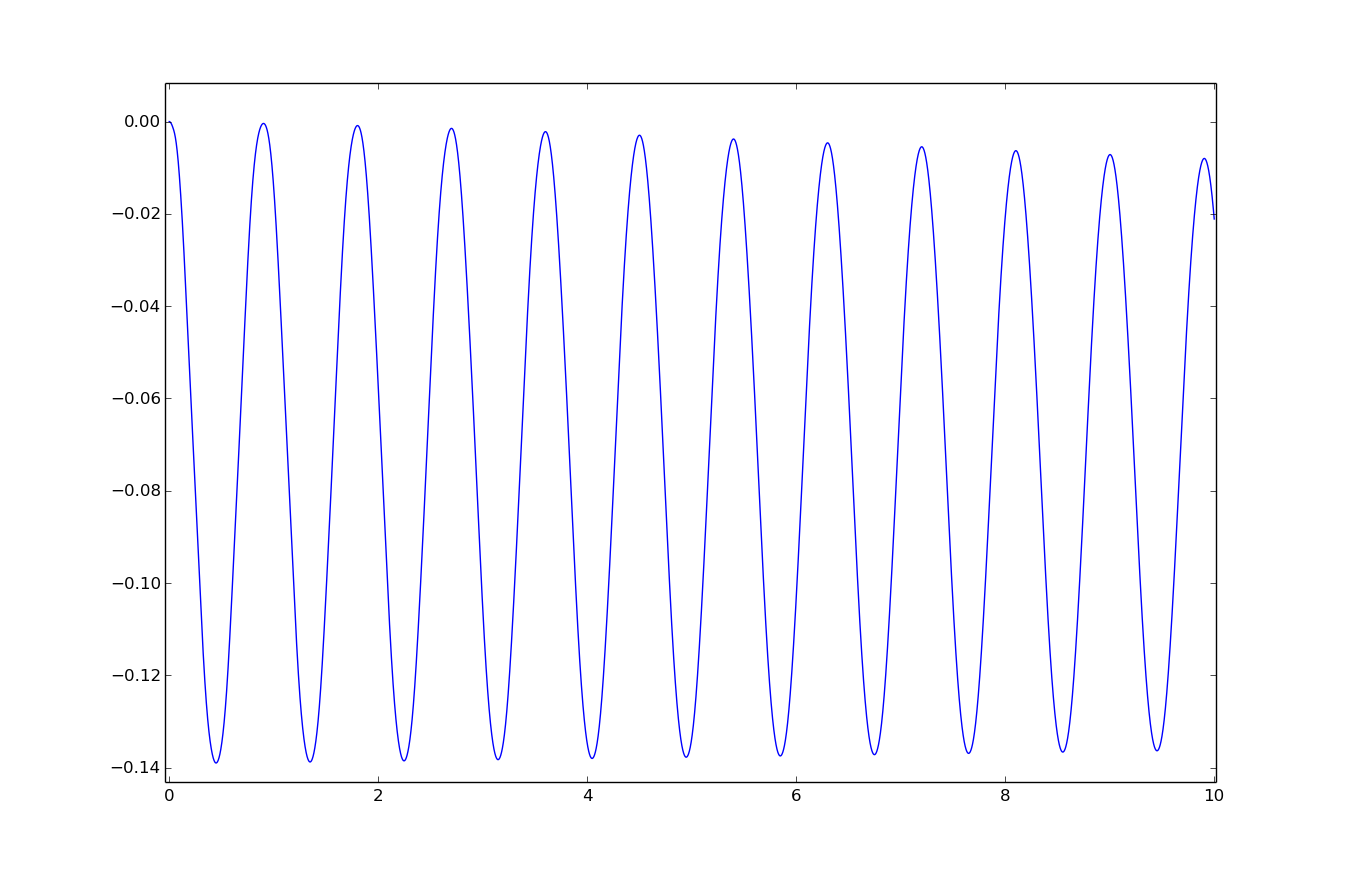
\includegraphics[width=\linewidth]{figures/CSM3/CSM3_Y_full}\caption{displacement y vs time}
\end{subfigure}
\begin{subfigure}[b]{0.5\linewidth}
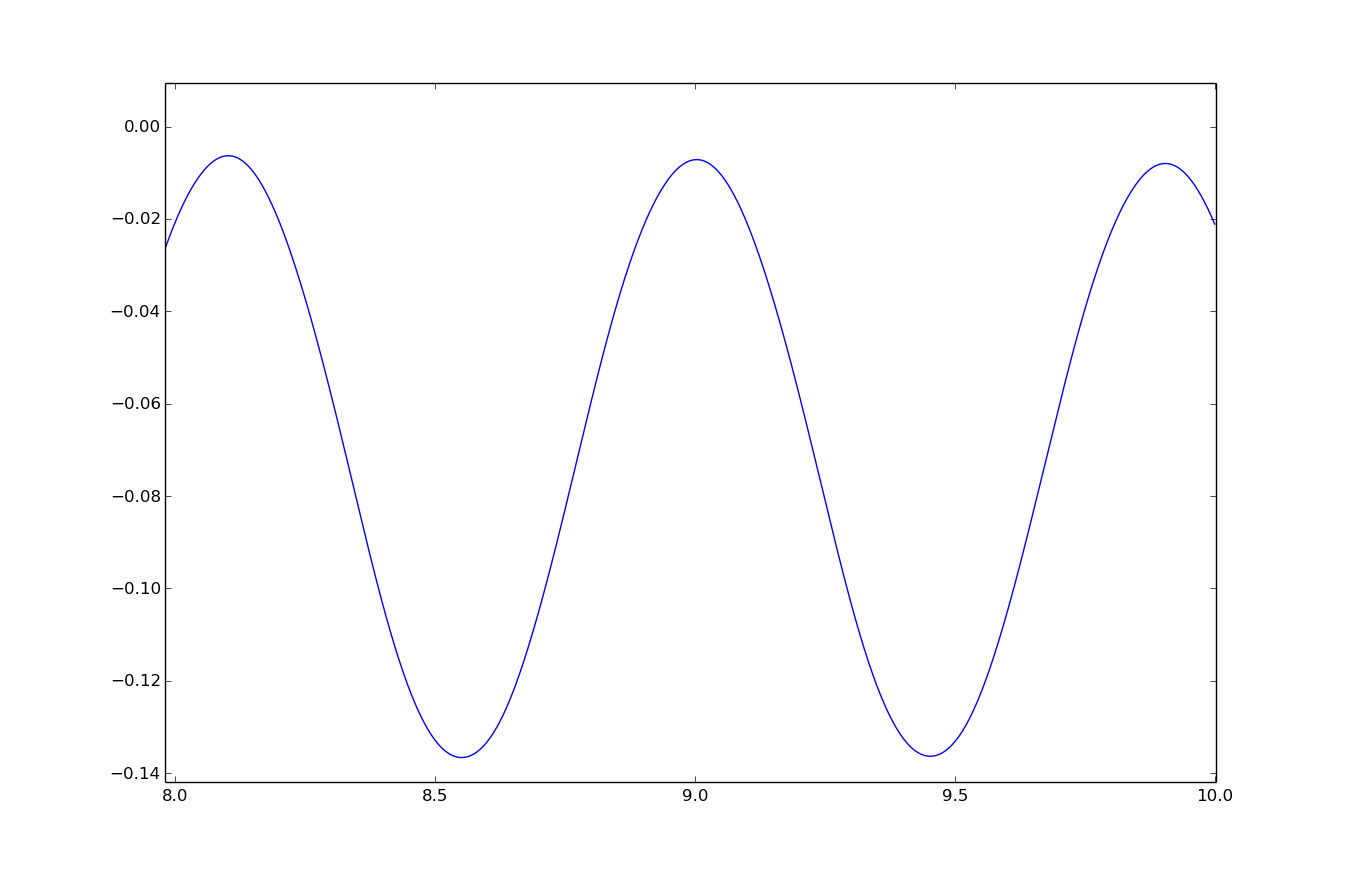
\includegraphics[width=\linewidth]{figures/CSM3/CSM3_2_y}\caption{displacement y vs time}
\end{subfigure}
\end{figure}
\clearpage

\subsection{FSI tests}
\begin{table}[!h]
\begin{center}
  \begin{tabular}{|l | l | l | l|} \hline
	Parameter & FS1 & FSI2 & FSI3 \\ \hline
    $\rho_f\, [10^3\frac{\text{kg}}{\text{m}^3}]$  & 1 & 1 & 1 \\   \hline
    $\nu_f\, [10^{-3}\frac{\text{m}^2}{\text{s}}]$ & 1 & 1 & 1 \\ \hline
    $\bar{v_0}$ & 0.2 & 1 & 2   \\ \hline \hline
    $\text{Re} = \frac{Ud}{\nu_f}$ & 20 & 100 & 200 \\ \hline
    \hline
  \end{tabular}
\end{center}
\end{table}

\begin{table}[!h]
\begin{center}
  \begin{tabular}{|l | l | l | l|} \hline
	Parameter & FSI1 & FSI2 & FSI3 \\ \hline
    $\rho_s \,[10^3\frac{\text{kg}}{\text{m}^3}]$  & 1 & 10 & 1 \\   \hline
    $\nu_s $ & 0.4 & 0.4 & 0.4 \\ \hline
    $\mu_s \,[10^{6}\frac{\text{m}^2}{\text{s}}]$ & 0.5 & 0.5 & 2   \\ \hline \hline
  \end{tabular}
\end{center}
\end{table}
\begin{center}
\begin{figure}[!h]
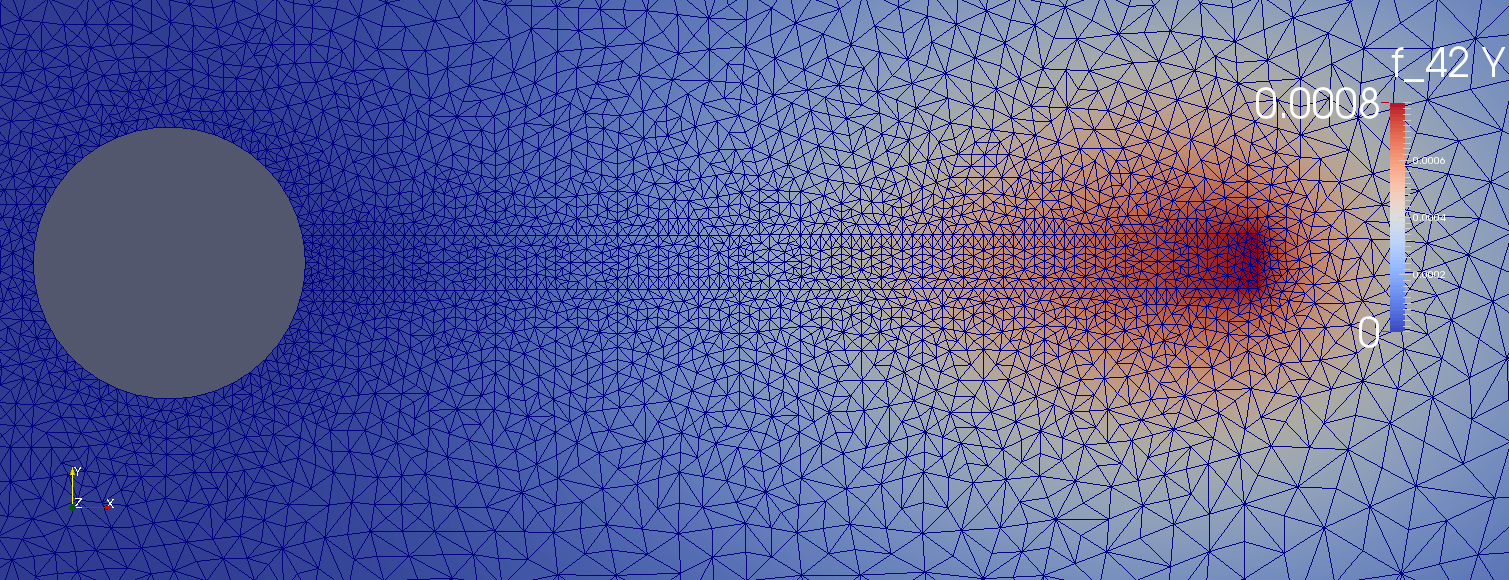
\includegraphics[width=\linewidth]{figures/FSI1_mesh_med}
\caption{Steady State displacement in y-direction for the FSI1 test case for the medium refinement version of the mesh. Note that the mesh around the structural part also has been slightly adjusted}
\end{figure}
\end{center}


\begin{table}[!h]
\begin{center}
  \begin{tabular}{|l | l | l | l | l | l|} \hline
	cells & dofs & $U_x$ of A $[10^{-3}]$ & $U_y$ of A $[10^{-3}]$ & Drag & Lift\\ \hline
    2698 & 15329 & 0.015596 & 0.74221 & 14.0876279441 & 0.756130219216 \\   \hline
    10792 & 60336 & 0.017738 & 0.77686 & 14.1777783843 & 0.763145083966 \\ \hline
    43168 & 239384 & 0.019824 & 0.79558  & 14.1869409712 & 0.758109277348  \\ \hline \hline
    \textbf{Ref.}  & & \textbf{0.0227} & \textbf{0.8209} & \textbf{14.295} & \textbf{0.7638}\\ \hline 
    \hline
  \end{tabular}	
\caption{Results for FSI1}
\end{center}
\end{table}

\begin{table}[!h]
  \begin{center}
  \begin{tabular}{|l | l | l | l | l | l|} \hline
	cells & dofs & $U_x$ of A $[10^{-3}]$ & $U_y$ of A $[10^{-3}]$ & Drag & Lift\\ \hline
   2698 & 15329 & $ -4.33 \pm 4.54$ & $ 1.40 \pm 29.96$ & $441.45 \pm 33.15 $ & $-2.30 \pm 178.00$\\   \hline
   10792 & 60336 & -4.84 $\pm$ 4.62 &  1.27 $\pm$ 31.74 & 469.11 $\pm$ 44.50 & 0.92 $\pm$ 97.27\\ \hline
   43168 & 239384 & $ $&  $ $ & $ $ & $ $   \\ \hline \hline
    \textbf{Ref.}  & & \textbf{-2.69} $\pm$ \textbf{2.53} & \textbf{1.48} $\pm$ \textbf{34.38} & \textbf{457.3} $\pm$ \textbf{22.66} & \textbf{2.22} $\pm$ \textbf{149.78}\\ \hline 
    \hline

  \end{tabular}
	  \caption{Results for FSI3}
  \end{center}
\end{table}
- note: Hron, Turek, $\Delta t = 0.0005$, we used $\Delta t = 0.0003$. \\ \\
\begin{figure}[!ht]
\begin{subfigure}[b]{0.5\linewidth}
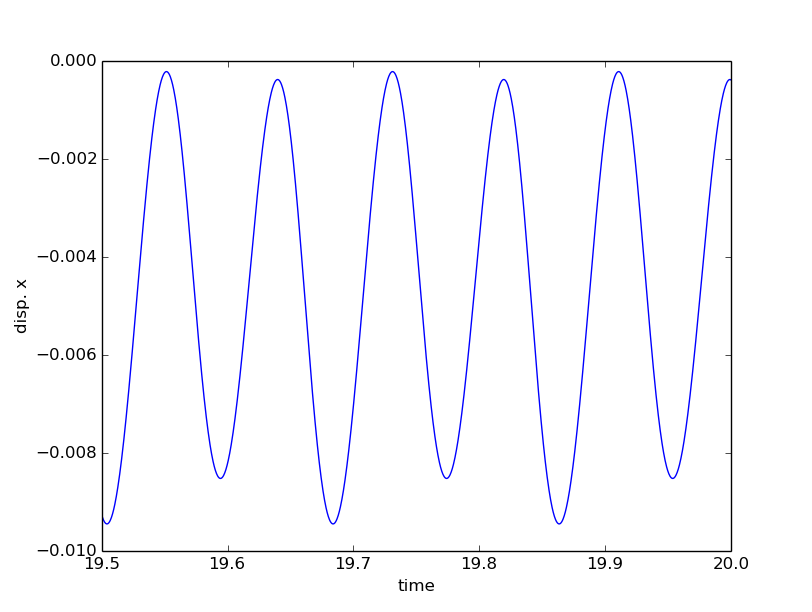
\includegraphics[width=\linewidth]{figures/FSI3/medium/X_disp}\caption{displacement x vs time}
\end{subfigure}
\begin{subfigure}[b]{0.5\linewidth}
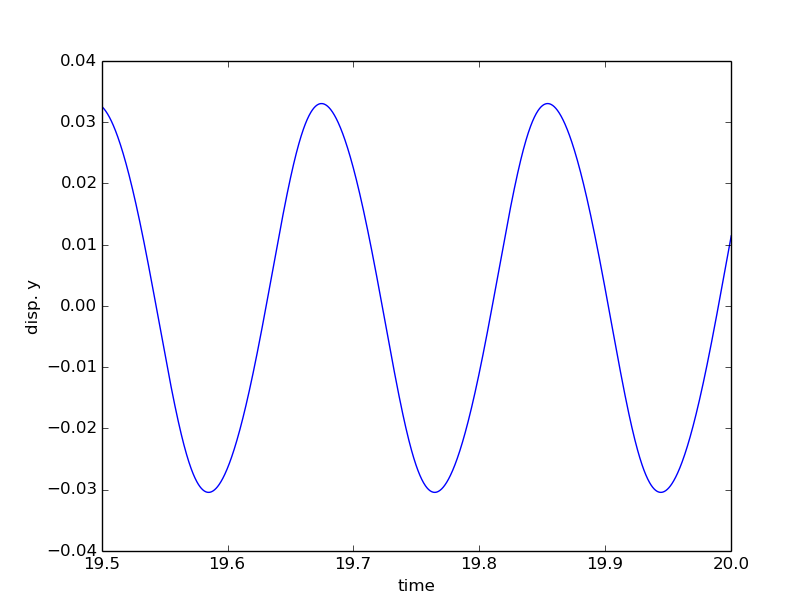
\includegraphics[width=\linewidth]{figures/FSI3/medium/Y_disp}\caption{displacement y vs time}
\end{subfigure}
\begin{subfigure}[b]{0.47\linewidth}
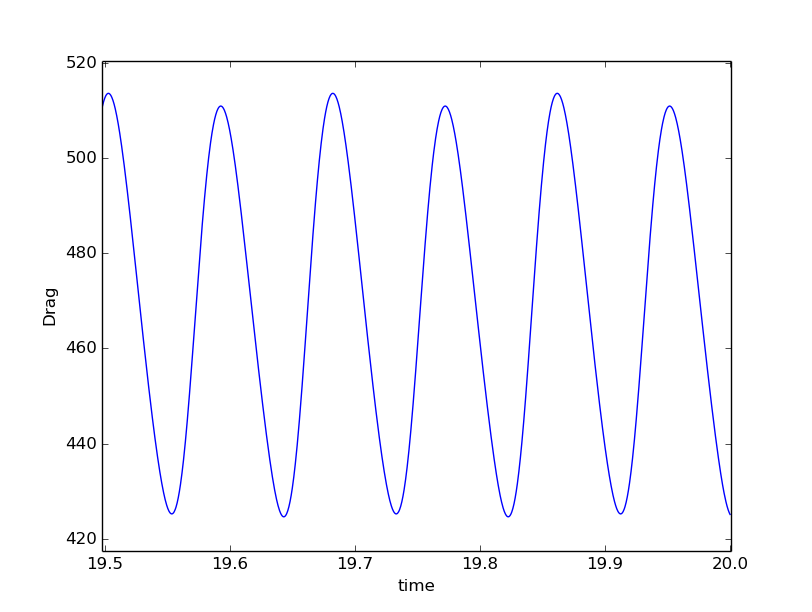
\includegraphics[width=\linewidth]{figures/FSI3/medium/Drag2}\caption{Drag vs time}
\end{subfigure}
\begin{subfigure}[b]{0.53\linewidth}
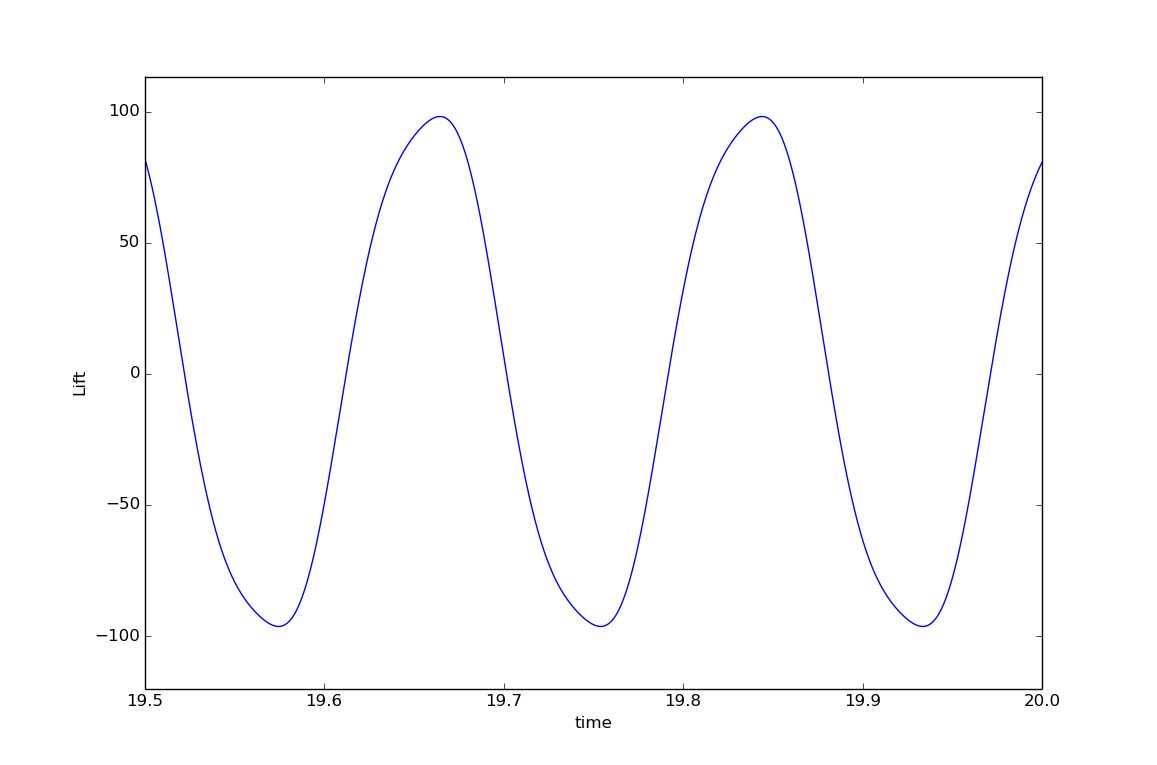
\includegraphics[width=\linewidth]{figures/FSI3/medium/Lift2}\caption{Lift vs time}
\end{subfigure}
\end{figure}

Numbers for FSI3:
Ux: Max = 0.0002099, Min = -0.008879 \\
Uy: Max = 0.03136, Min = -0.02856 \\
Drag: Max = 474.6, Min = 408.3 \\
Lift: Max = 175.7, Min = -180.3 (174.4, -177.0\\

Frequency, 0.1795 /s for medium mesh.
\begin{center}
\begin{figure}[!ht]
\begin{subfigure}[b]{0.5\linewidth}
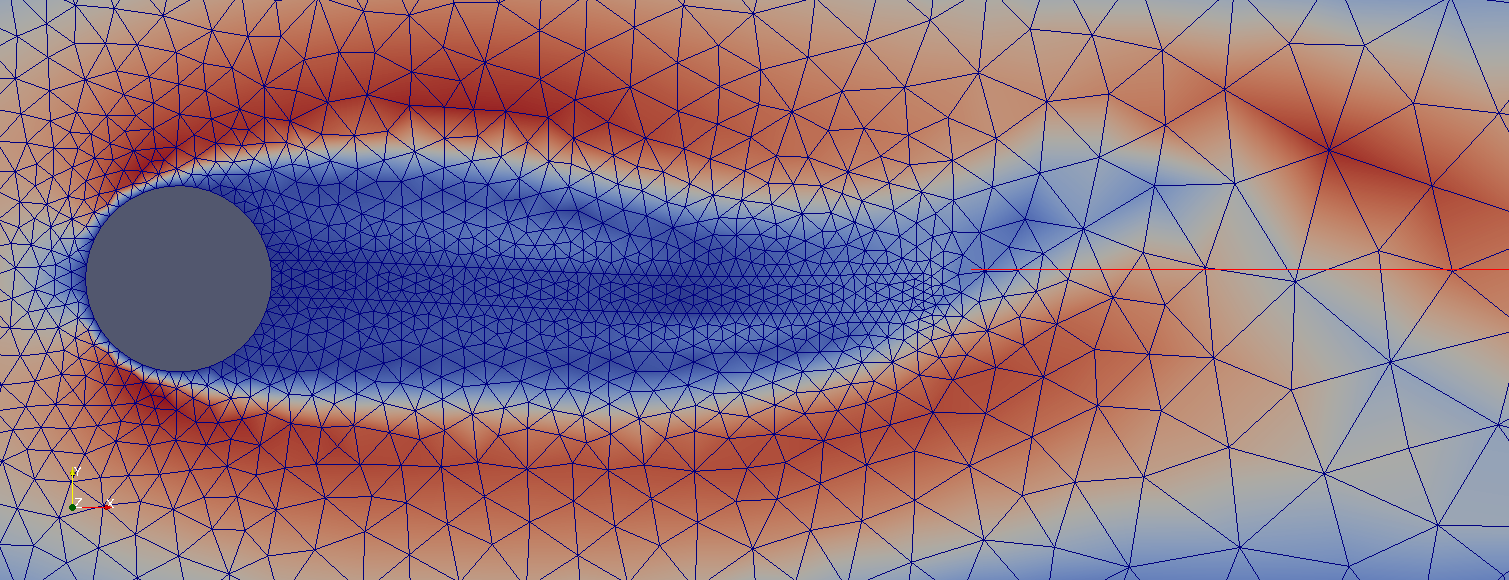
\includegraphics[width=\linewidth]{figures/FSI3/coarse/FSI_mesh_1}
\caption{t=10.88}
\end{subfigure}
\begin{subfigure}[b]{0.5\linewidth}
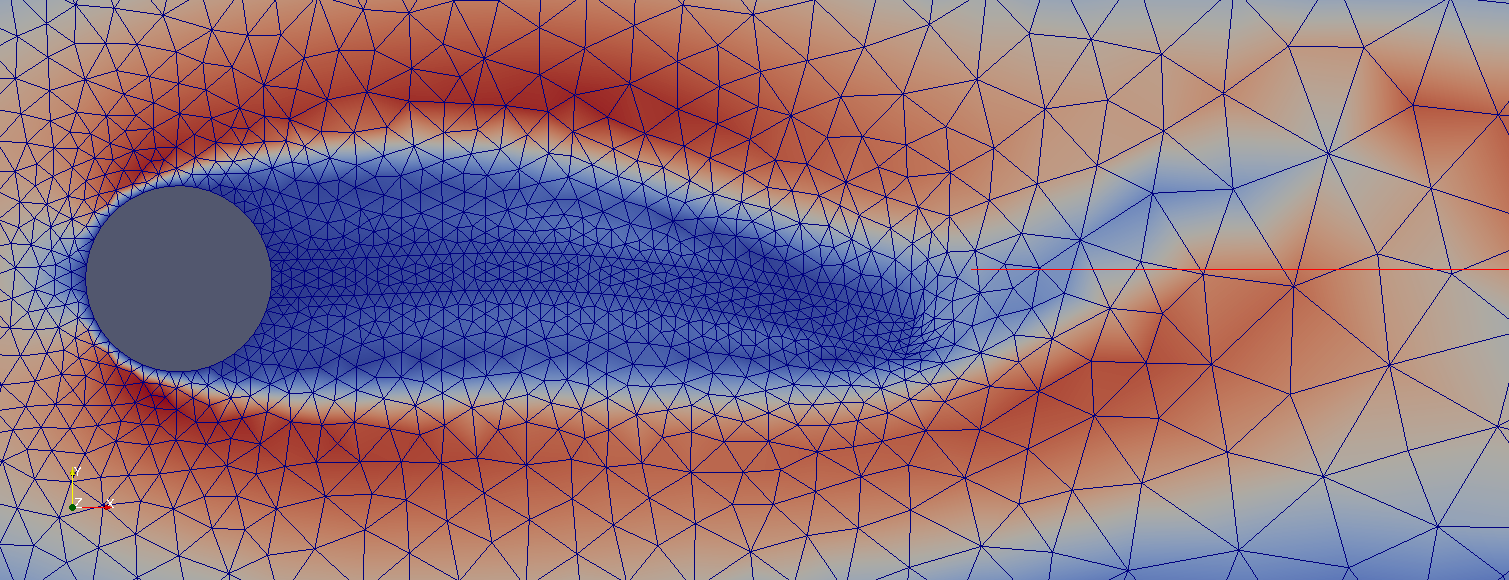
\includegraphics[width=\linewidth]{figures/FSI3/coarse/FSI_mesh_2}
\caption{t=10.91}
\end{subfigure} \\
\begin{subfigure}[b]{0.5\linewidth}
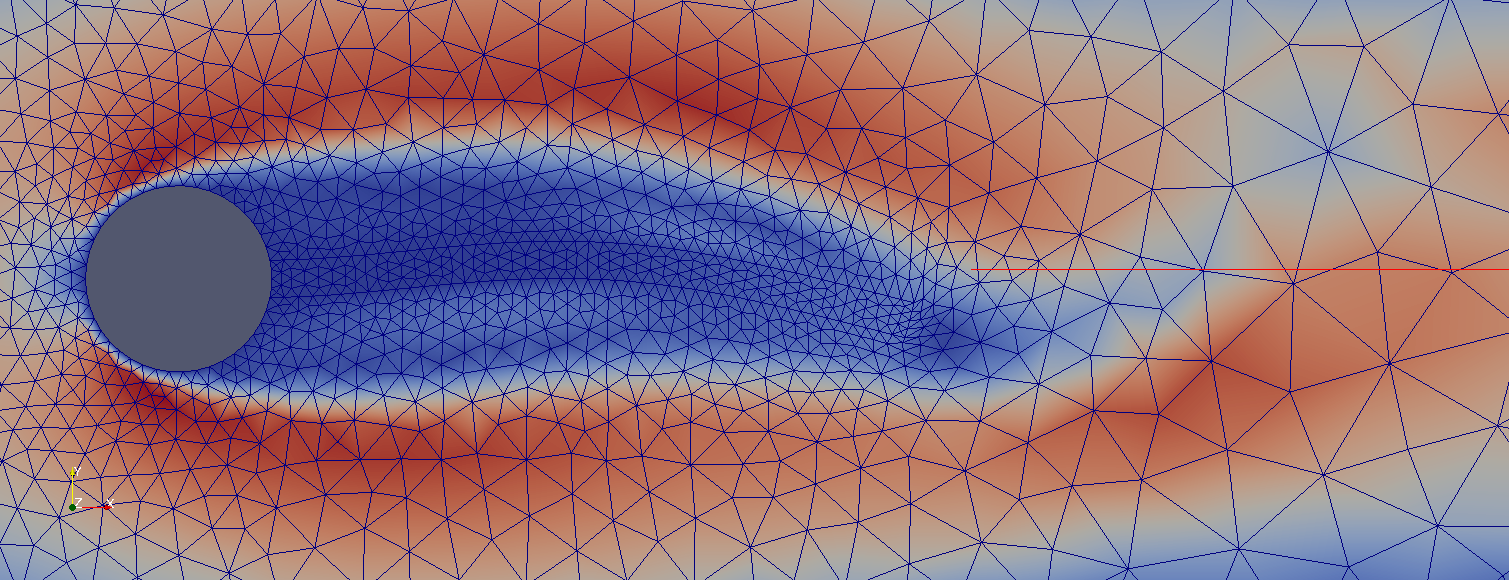
\includegraphics[width=\linewidth]{figures/FSI3/coarse/FSI_mesh_3}
\caption{t=10.94}
\end{subfigure}
\begin{subfigure}[b]{0.5\linewidth}
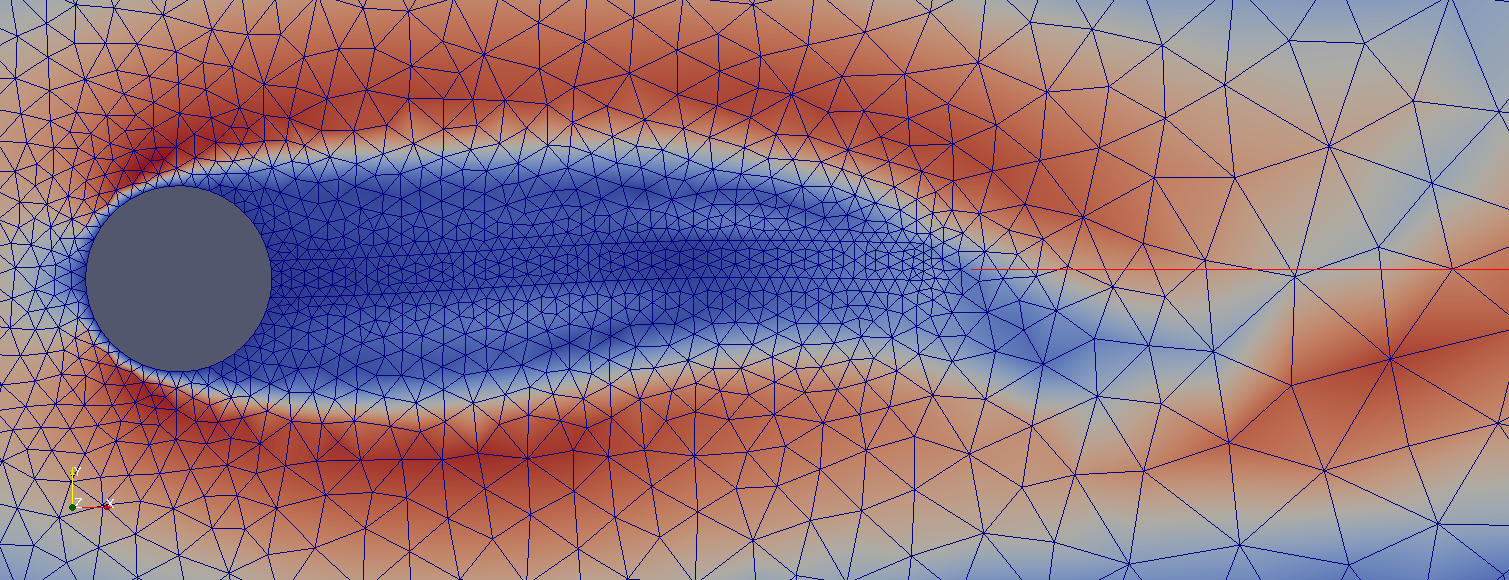
\includegraphics[width=\linewidth]{figures/FSI3/coarse/FSI_mesh_4}
\caption{t=10.97}
\end{subfigure} \\
\begin{subfigure}[b]{0.5\linewidth}
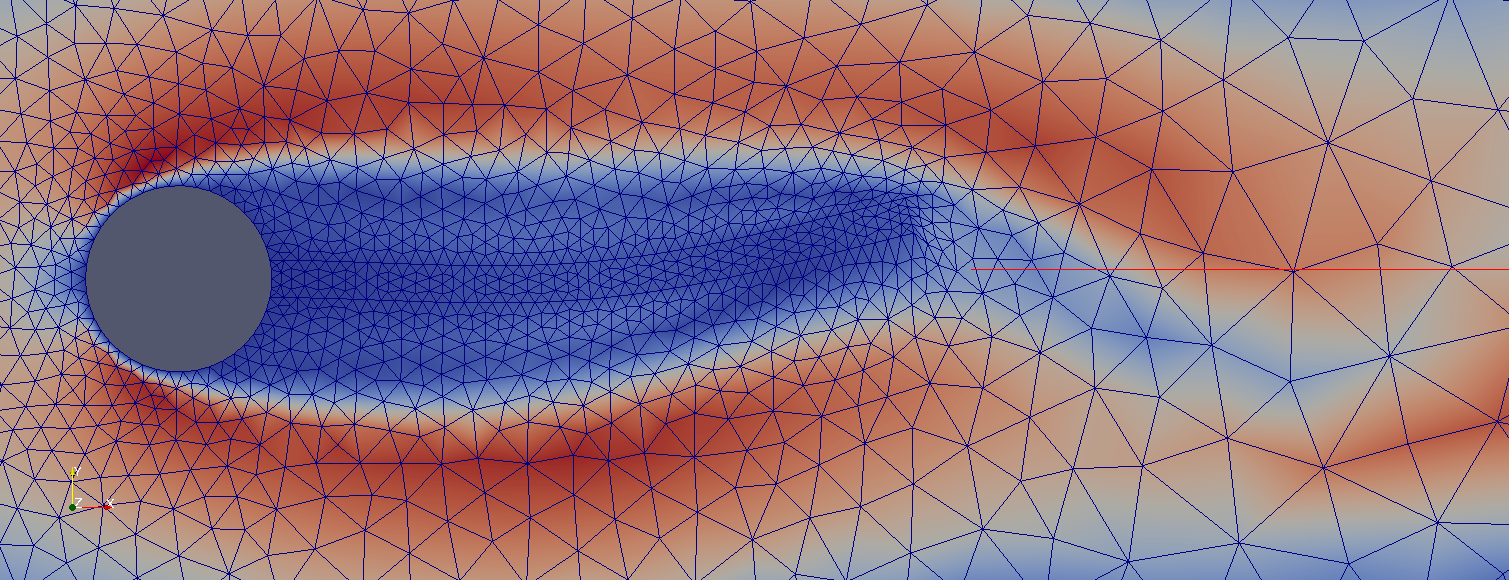
\includegraphics[width=\linewidth]{figures/FSI3/coarse/FSI_mesh_5}
\caption{t=11.00}
\end{subfigure}
\begin{subfigure}[b]{0.5\linewidth}
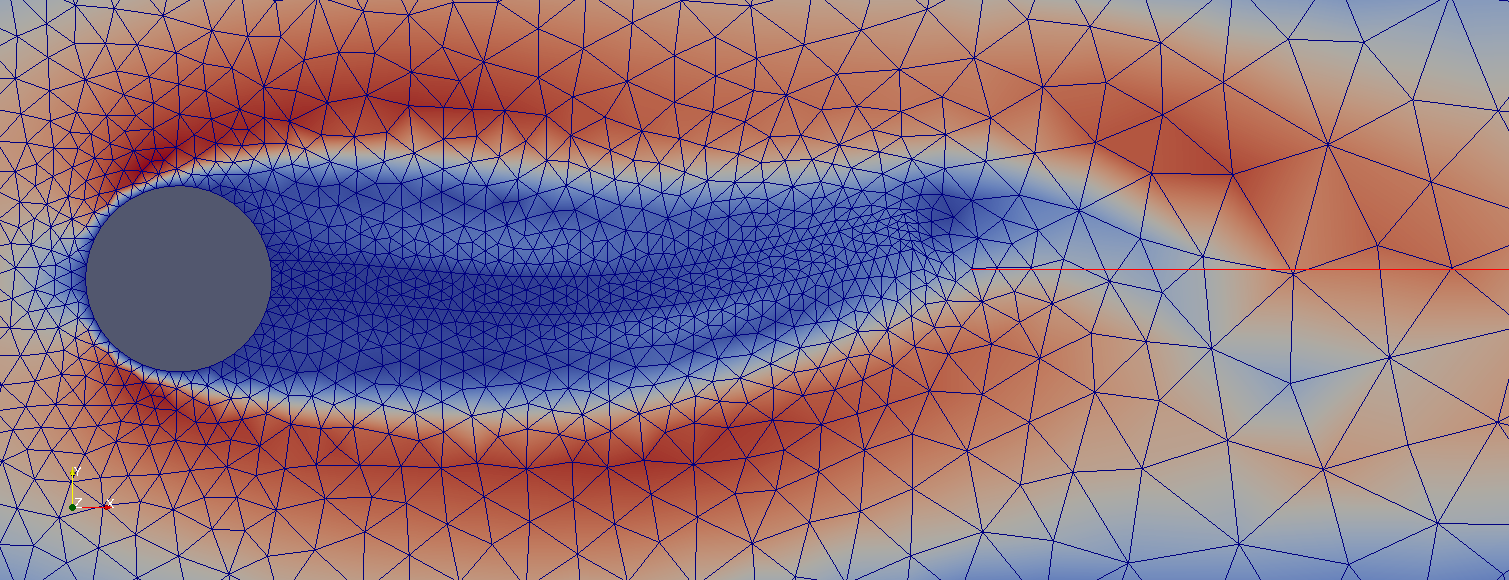
\includegraphics[width=\linewidth]{figures/FSI3/coarse/FSI_mesh_6}
\caption{t=11.03}
\end{subfigure}
\caption{The colormap shows the magnitude of the velocity around the flag at six different states of time in fully developed flow on the coarsest mesh. Maximum velocity reaches 4.37. The mesh consists of a smooth curve at the interface, and the domains are separated beforehand in FEniCS}
\end{figure}
\end{center}
\clearpage



\section{Fluid Structure Interaction using the Finite Element method}
The solver was implemented from scratch in Python using the DOLFIN library. FSI solvers within the FEniCS framework exists, e.g. under Unicorn or CBC.twist. For instance, Selin \cite{Seli11} implemented a partitioned solver in FEniCS in his PhD-thesis, using the already existing modules for solving fluid flow and structural deformations separately (CBC.Flow and CBC.Twist). With the implementation presented here, it will be easier to adjust the solver with respect to the model. The equations can be changed whether we want the spinal cord to be porous, elastic, poroelastic or viscoelastic. The use of two separate solvers is also problematic for the monolithic approach, when all equations should be solved simultaneously. On the other hand, solvers implemented by experienced and skilled research groups will probably be a lot more efficient and should already have been validated. 
\\
\\
In the rest of this section, we give a brief explanation to the mathematics and implementation in FEniCS. In the previous example we saw the close link between code and mathematics. :
\begin{align*}
a(\mathbf{v},\Phi) = (\nabla \mathbf{v}, \nabla \Phi)_\Omega \\
L(\mathbf{v}) = (\mathbf{f},\Phi)_\Omega
\end{align*}
Translates to
\begin{center}
\begin{cverbatim}
a = inner(grad(v),grad(phi)*dx
L = inner(f,phi)*dx
\end{cverbatim}
\end{center}
In deriving variational forms, we try to keep this close link by recalling the symbols used for velocity ($\mathbf{v}$), total displacement ($\mathbf{U}$), pressure ($p$), and mesh velocity, ($\mathbf{w}$). Also recall that in the solid the mesh moves exactly with the velocty of the structure so $\mathbf{w}_s = \mathbf{v}_s$
\\
\subsection{Temporal discretization}
In order not to overload this thesis with notation and superscripts, we have used the notation $\mathbf{v} := \mathbf{v}^{n+1}$ to denote the value of a function at the next time-step. Similarly, we define $\mathbf{v^{(1)}} := \mathbf{v}^n$ to denote the (known) value of a function at the present time step. 
\\
\\
The total displacement $\mathbf{U}$ can be expressed as a function of the displacement from the previous time step, $\mathbf{U}^{(1)}$, and the mesh velocity $\mathbf{w}$. We have used an implicit scheme in time, i.e, $(\pdi{\mathbf{v}}{t})^{n+1} \approx \frac{\mathbf{v}^{n+1}-\mathbf{v}^{n}}{\Delta t} $, and $\mathbf{U} = \mathbf{U}^{(1)} + \Delta t \mathbf{w}$. 







\subsection{Spatial discretization}
When dealing with nonlinear equations, such as the Navier-Stokes equation, \textit{linearization} is needed in order to solve the equations. In the nonlinear terms, we simply replace one (or more) of the unknown $\mathbf{v}$'s with a "guess" to get an equation linear in $\mathbf{v}$. This guess is denoted as $\mathbf{v}^{(0)}$. Since we have three unknown functions, we use a mixed function space with three function spaces, $\Phi$, $\eta$ and $\Psi$. In the fluid we multiply the momentum equation with $\Phi$, the continuity equation with $\eta$ and the equation for mesh velocity with $\Psi$ and integrate over the domain in its \textit{current} configuration, $\Omega^t$. In the fluid, this yields
\begin{align}
\frac{\rho_f}{\Delta t}(\mathbf{v},\Phi)_{\Omega_f} + \rho_f(((\mathbf{v}-\mathbf{w})\cdot \nabla) \mathbf{v}^{(0)}, \Phi)_{\Omega_f^t} - (p,\nabla \cdot \Phi)_{\Omega_f^t} + 2\mu_f(\epsilon(\mathbf{v}), \nabla \Phi)_{\Omega_f^t} = \\ 
\frac{\rho_f}{\Delta t}(\mathbf{v}^{(1)},\Phi)_{\Omega_f^t} - (\sigma_f(p,\mathbf{v})\cdot \mathbf{n}, \Phi)_{\partial \Omega_f^t} - (\sigma_f(p,\mathbf{v}) \cdot \mathbf{n}_f, \Phi)_{\Gamma^t} \label{VarMom}
\end{align}
\begin{align}
-(\nabla \cdot \mathbf{v},\eta)_{\Omega_f^t} = 0 \label{VarCon}
\end{align}
\begin{align}
\Delta t(\nabla \mathbf{w}, \nabla \Psi)_{\Omega_f^t} = - (\nabla \mathbf{U}^{(1)}, \nabla \Psi)_{\Omega_f^t} & + ([\nabla \mathbf{U}^{(1)} + \Delta t \nabla \mathbf{w}] \cdot \mathbf{n}, \Psi)_{\Omega_f^t} \\ 
& + ([\nabla \mathbf{U}^{(1)} + \Delta t \nabla \mathbf{w}] \cdot \mathbf{n}_f, \Psi)_{\Gamma^t} \label{VarMesh}
\end{align}
\\
And in the solid
\begin{align}
\frac{\rho_s}{\Delta t}(\mathbf{v},\Phi)_{\Omega_s} + \Delta t (\sigma_s (\mathbf{v}), \nabla(\Phi))_{\Omega_s} & = \frac{\rho_s}{\Delta t}(\mathbf{v}^{(1)},\Phi)_{\Omega_s} - (\sigma_s(\mathbf{U}^{(1)}), \nabla \Phi)_{\Omega_s} \\
& - ([\sigma_s(\mathbf{U}^{(1)}) + \Delta t \sigma_s(\mathbf{w})]\cdot \mathbf{n}, \Phi)_{\partial \Omega_s^t} \\
& - ([\sigma_s(\mathbf{U}^{(1)}) + \Delta t \sigma_s(\mathbf{w})]\cdot \mathbf{n}_s, \Phi)_{\Gamma^t} \label{VarMom2}
\end{align}
\begin{align}
\frac{1}{\delta}(\mathbf{v},\Psi)_{\Omega_s} - \frac{1}{\delta}(\mathbf{w},\Psi)_{\Omega_s} = 0 \label{VarMesh2}
\end{align}
The parameter $\delta $ should be small and ensures the importance of $\mathbf{v_s} = \mathbf{w_s}$ inside the solid. On the interface, we have distinguished between the normal vector with respect to the fluid and solid domain. In general $\mathbf{n}_f = -\mathbf{n}_s$. To be able to set up and assemble the matrices for this system, the equations should be added to form one bilinear form and one linear form.



 
\subsection{A discussion on functionspaces}
We have previously defined the $L^2$ (def. \ref{|l2}) and $H^1$ (def. \ref{H1}) spaces, as well as the linear continuous galerkin basis functions (section \ref{FinEle}). In order to have a well posed-problem, we need a triple $(\Phi,\eta, \Psi)$ to satisfy a few given conditions. In the following, a brief justification of the choice of function spaces used in this study are given. \\
\\
For the incompressible Navier-Stokes equations, much of the mathematical theory and understanding have been developed by investigation of the simplified Stokes flow where the acceleration term is neglected in the momentum equation, that is
\begin{align}
-\mu\nabla^2\mathbf{u} + \nabla p = \mathbf{F}
\end{align} Numerous possible pairs $(\Phi, \eta)$ have been proposed over the years since the first report by Taylor and Hood \cite{Tayl73}. The discretization used by Taylor and Hood consists of quadratic piecewise polynomials for the velocity components and linear piecewise polynomials for the pressure and is still a very popular choice of basis functions. These types of elements are often referred to as Taylor-Hood elements or simply just P2-P1 elements. 
\\
\\
As mentioned earlier, the final step in the finite element method consists of solving a linear system of equations. In the case of Stokes equations with body forces $\mathbf{f}$, a matrix system on the following form needs to be solved
\begin{align}
\begin{bmatrix}
\mathbf{A} & \mathbf{B} \\
\mathbf{B}^T & \mathbf{0}
\end{bmatrix}
\begin{bmatrix}
\mathbf{v} \\
\mathbf{p}
\end{bmatrix}   = 
\begin{bmatrix}
\mathbf{f} \\
\mathbf{0}
\end{bmatrix}
\end{align}
Which means that
\begin{align}
\mathbf{A}\mathbf{v} + \mathbf{B}\mathbf{p} = \mathbf{f} \label{MatrixMom}
\end{align}
\begin{align}
\mathbf{B}^T \mathbf{v} = \mathbf{0}   \label{MatrixCon}
\end{align}
To get an expression for $\mathbf{v}$, we multiply \eqref{MatrixMom} with $\mathbf{A}^{-1}$ to obtain
\begin{align}
\mathbf{v} = \mathbf{A}^{-1}(\mathbf{f} - \mathbf{B}\mathbf{p})
\end{align}
And insert this expression into \eqref{MatrixCon} to get an equation only involving the pressure
\begin{align}
\mathbf{B}^T \mathbf{A}^{-1}(\mathbf{f} - \mathbf{B}\mathbf{p}) = \mathbf{0}
\end{align}
or
\begin{align}
\mathbf{B}^T\mathbf{A}^{-1}\mathbf{B}\mathbf{p} = \mathbf{B}^T\mathbf{A}^{-1}\mathbf{f}
\end{align}
For the solution to be unique, the matrix $\mathbf{B}^T\mathbf{A}^{-1}\mathbf{B}$ often reffered to as the \textit{Schur complement} needs to be non-singular. A necessary and sufficient condition for this is that Ker($\mathbf{B}$) = \{0\}, or
\begin{align}
\sup_{\mathbf{v}_h}\int p_h \nabla \cdot \mathbf{v}_h > 0
\end{align}
For all discrete pressures $p_h \neq 0$. 
This ensures solvability. For convergence, the famous Babuska-Brezzi (BB), or inf-sup condition needs to be satisfied \cite{Brez12}
\begin{align}
\inf_{p_h}\sup_{\mathbf{v}_h} \frac{\int_{\Omega}p_h \nabla \cdot \mathbf{v}_h}{||\mathbf{v}_h||_1 ||p_h||_0} \geq D > 0
\end{align}
Where D is a constant independent of the mesh resolution. 
\\
\\
Provided this condition is satisfied the following error estimate should hold for the Stokes equations
\begin{align}
||\mathbf{v}_h-\mathbf{v}||_1 + ||p_h - p||_0 < C(h^k||\mathbf{v}||_{k+1} + h^{l+1}||p||_{l+1})
\end{align}
Where k and l are the degrees of polynomials used for velocity components and pressure, respectively. To obtain optimal convergence for the solution the polynomial degree should be one higher for the velocity components than for the pressure, that is, $k = l+1$. For instance, using P3-P1 elements, computer resources are "wasted" by introducing more degrees of freedom (dofs) without improving convergence. Several choices of element type combinations, for instance Linear elements (P1) both for velocity and pressure do not satisfy the BB condition, and as a consequence unphysical oscillations in pressure can be seen. 
\\
\\
Elements not satisfying the BB condition can be used if a proper stabilization is introduced. Due to the drastical reduction in dofs, P1-P1 elements are often used when large systems are solved for instance in commercial software. This combination is default in COMSOL, while for 3D problems in FLUENT, a slightly different element, the "mini-element" is used as first developed by Fortin \cite{Fort81}. This element is linear but with an extra degree of freedom known as a bubble in the center. 
\\
\\
In this study, P2-P1 elements are used for the material velocity and pressure. However, a function space is also needed for the domain velocity, $\mathbf{w}$. As discussed by Quaini \cite{Quai09}, P1-elements for the domain velocity will ensure the transformation of straight lines in the new domain. In the fluid momentum equation, the funciton $\mathbf{w}$ is only used in the term $((\mathbf{v}-\mathbf{w})\cdot \nabla) \mathbf{v}^{(0)}$ and since $\mathbf{v}$ is a polynomial of degree 2, $\mathbf{v}-\mathbf{w}$ will also be a polynomial of degree 2. Therefore, the 


\subsection{Treatment of boundary conditions}
In addition to the boundary conditions described in the original benchmark paper from Turek and Hron, homogenuous Dirichlet conditions are prescribed to the mesh displacement velocity on the domain boundary, i.e 
\begin{align} 
\mathbf{w} = 0 \text{ on } \partial \Omega_f^t \cup \partial \Omega_s^t
\end{align}
Except for the fluid velocity on the outlet, the domain boundaries (not interface) have prescribed Dirichlet conditions on both $\mathbf{u}$ and $\mathbf{w}$. Therefore the test functions $\Phi$ and $\Psi$ will be zero on these boundaries. \\ \\
If we add all the equations in the previous section together, the contributions to the boundary integral on the interface gives:
\begin{align}- (\sigma_f(p,\mathbf{v}) \cdot \mathbf{n}_f, \Phi)_{\Gamma^t} - ([\sigma_s(\mathbf{U}^{(1)}) + \Delta t \sigma_s(\mathbf{w})]\cdot \mathbf{n}_s, \Phi)_{\Gamma^t}
\end{align}
By leaving this out of the variational form, we weakly impose
\begin{align} \sigma_f(p,\mathbf{v}) \cdot \mathbf{n} = \sigma_s(\mathbf{U}) \cdot \mathbf{n}
\end{align}
On the interface. The choice of $\mathbf{n}$ ($\mathbf{n} = \mathbf{n}_f$ or $\mathbf{n} = \mathbf{n}_s$) is arbitrary, but the same for each side of the equation. \\
\\
Because we use the same function for fluid velocity and solid velocity, the no-slip condition is naturally incorporated for the fluid on the structure
\begin{align}
\mathbf{v}_f = \mathbf{v}_s \text{ on } \Gamma^t
\end{align}
Because the functions $\mathbf{v}_f$ and $\mathbf{v}_s$ share nodes on the interface.
\\
\\
The additional equation for $\mathbf{w}$ in the fluid also gives rise to boundary conditions on $\nabla \mathbf{U}\cdot\mathbf{n}$ on the interface. To this end we set 
\begin{align}
\nabla \mathbf{U} \cdot \mathbf{n} = 0
\end{align}
and rather let the parameter $\delta$ underline the importance of $\mathbf{w} = \mathbf{v}$ \textit{inside} the solid, whereas $\mathbf{w}$ in the fluid should just ensure a smooth mesh displacement. \\
\\
On the outlet, we assign the stress-free condition $\sigma_f(p,\mathbf{v}) \cdot \mathbf{n} = 0$ so the boundary integral also vanish on the outlet for the momentum equation in the fluid. 
\\
\\
This means that all integrals involving boundaries will vanish in the variational form. The Dirichlet conditions are imposed in FEniCS as previously described.


\subsection{FSI in FEniCS}
There will be some changes and a great leap in complexity compared to the previous example using FEniCS. The main differences and additions are explained here. One thing to highlight is the always ongoing changes and updates in the dolfin library. Therefore, if a solver was to be used by someone other than the writer, it will constantly need updates and fixes. This thesis do not intend to present a solver with great complexity and many options, but rather outline the most important lines of code and explain difficulties behind the FSI problem in FEniCS. The explanation here intends that a reader somewhat familiar with FEniCS should be able to implement such a code within a short amount of time. 
\\
\\
The computational mesh is constructed in gmsh with a straight boundary dividing the fluid and the solid. This way, the class MeshFunction can be utilized by dividing the mesh in two subdomains. We now assume we have classes describing the solid and fluid region, implemented with functions simliary to the boundary functions in the Poisson example. 
\begin{cverbatim}
mesh = Mesh('FSI_mesh.xml')
SD = MeshFunction('uint', mesh, mesh.topology().dim())
SD.set_all(0)
Elastic().mark(SD,1)
\end{cverbatim}
where 
\begin{cverbatim}
class Elastic(SubDomain):
	def inside(self,x,on_bnd):
		# returns True if vector x in solid.
\end{cverbatim}
'uint' means that the MeshFunction has values of nonnegative integers. The last argument ensures the MeshFunction to have the same dimension as the mesh. \\
Using the MeshFunction, the fluid domain have been marked 0, and the solid domain have been marked 1. Integration over the two domains can be separated by passing this number to dx in the variational formulation. A similar class, the FacetFunction
\begin{cverbatim}
boundaries = FacetFunction("size_t",mesh)
\end{cverbatim}
is used to mark the boundaries and, if needed, separate integration over specific parts of the boundary.
\\
\\'uint' means that the MeshFunction has values of nonnegative integers. 'size\_t' means the same for the FacetFunction. The last argument to MeshFunction ensures the MeshFunction to have the same dimension as the mesh. 
\\ \\	
We need a function spaces for all three testfunctions, corresponding to $\mathbf{v}, p$ and $\mathbf{w}$, and in this case we can use a handy FEniCS class to create a mixed function space. Test -and trial functions should also be created from this mixed space.
\begin{cverbatim}
V = VectorFunctionSpace(mesh,'CG',2)
P = FunctionSpace(mesh,'CG',1)
W = VectorFunctionSpace(mesh,'CG', 1)
VPW = MixedFunctionSpace([V,P,W])
v,p,w = TrialFunctions(VPW)
phi,eta,psi = TestFunctions(VPW)
\end{cverbatim}
All Dirichlet boundary conditions need to be specified, and the functions need to be in the space of the respective trial function where the condition is set. For instance, the top boundary of the domain have been marked 2 with the FacetFunction, and we want to presribe the no-slip condition on the fluid velocity.
\begin{cverbatim}
noslip = Constant((0.0,0.0))
bcv2 = DirichletBC(VPW.sub(0),noslip,boundaries,2) # Top
\end{cverbatim}
All the Dirichlet boundary conditions are put together in a list, bcs.\\ \\
When the Mesh -and FacetFunctions have been properly marked, we need to map the information from these classes to the different measures, dx, ds and dS representing integration over cells, exterior facets and interior facets, respectively. This is done by:
\begin{cverbatim}
dS = Measure('dS')[boundaries]
dx = Measure('dx')[SD]
ds = Measure('ds')[boundaries]

dx_f = dx(0,subdomain_data=SD)
dx_s = dx(1,subdomain_data=SD)
\end{cverbatim}
The last two lines simplifies the integrands in the variational form and make it more clear which expressions are to be used in the fluid domain and which should be used in the solid domain.
\\
Sometimes, it can be convinient to define the constants used in FEniCS as instances of the class Constant, to avoid re-compiling if the value of the constant is changed. e.g.
\begin{cverbatim}
dt = 0.0003
k = Constant(dt)
\end{cverbatim}
We can now attention our focus to the variational form. Regular Python functions can be used in the variational formulation, and by defining these two
\begin{cverbatim}
def sigma_s(U):
	return 2*mu_s*sym(grad(U)) + lamda*tr(sym(grad(U)))*Identity(2)

def eps(v):
	return 2*mu_f*sym(grad(v))
\end{cverbatim}
To be able to start the simulation some initial conditions are needed, and by setting
\begin{cverbatim}
U = Function(W)
v1 = Function(V)
v0 = Function(V)
\end{cverbatim}
The initial conditions are simply set to be zero both for velocity and displacement.
\\
\\
The variational form is very similar to the mathematics. We define the bilinear and linear forms, a and L, for each separate equation, momentum, continuity and the movement of the domain in both the fluid and solid domain (except for continuity in the solid). For instance, aMF will denote the bilinear form, a, for the momentum equation in the fluid.
\begin{cverbatim}
# FLUID
aMF = rho_f/k*inner(v,phi)*dx_f + \
	rho_f*inner(grad(v0)*(v-w),phi)*dx_f - \
	 inner(p,div(phi))*dx_f + \
	2*mu_f*inner(eps(v),grad(phi))*dx_f

LMF = rho_f/k*inner(v1,phi)*dx_f

aCF = -inner(div(v),eta)*dx_f

aDF = k*inner(grad(w),grad(psi))*dx_f
LDF = -inner(grad(U),grad(psi))*dx_f

aF = aMF + aCF + aDF
LF = LMF + LDF

# SOLID
aMS = rho_s/k*inner(v,phi)*dx_f + \
	k*inner(sigma_s(v),grad(phi))*dx_f

LMS = rho_s/k*inner(v1,phi)*dx_f - \
	inner(sigma_s(U),grad(phi))*dx_f

aDS = 1/delta*inner(u,w)*dx_f - \
	1/delta*inner(d,w)*dx_f


aS = aMS + aDS
LS = LMS

\end{cverbatim}
We can now add the forms together to obtain one biliear and one linear form
\begin{cverbatim}
a = aS + aF 
L = LS + LF
\end{cverbatim}
Before the time loop starts we define a function for holding the solution:
\begin{cverbatim}
VPW_ = Function(VPW)
\end{cverbatim}
This function will consist of all values for $\mathbf{v}$, $p$ and $\mathbf{w}$.
\\
\\
The time loop runs until the current time exceeds the specified end time, T. The forms change in time, and thus needs to be assembled to be updated to use the correct values for $\mathbf{v}^{(1)}, \mathbf{w}^{(1)}, \mathbf{U}^{(1)}$ and $\mathbf{v}^{(0)}$. The linear form needs an update each time step, while the bilinear form needs to be updated every single iteration inside the time loop. For the iterative method, we have chosen the Picard iteration based on the simplicity of the algorithm compared to Newton's method, especially when dealing with a mixed function space consisting of three separate spaces. The iteration runs until the $L^2$ norm of $(\mathbf{v}-\mathbf{v}^{(0)})$ is less than a given number, $\tau$, or if the number of iterations becomes to large. 

\begin{cverbatim}
while t < T:
	...
	b = assemble(L)
	...
	while error > tau and k_iter < max_iter:
		A = assemble(a)
		A = ident.zeros()
		[bc.apply(A,b) for bc in bcs]
		solve(A,VPW_.vector,b,'lu')
		v_,p_,w_ = VPW_.split(True)
		eps = errornorm(v_,v0,degree_rise=3)	
		k_iter += 1
		
		v0.assign(v_)
\end{cverbatim}
The second statement within the iteration loop is needed because the lack of an equation for $p$ within the solid. The \textit{ident.zeros()} function replaces zeros with ones on the diagonal of the matrix block, and the solution vector for $p$ will be zero inside the solid. In FEniCS, a Function has to be defined over the whole mesh, and adjusting the linear system as described is a way to overcome this issue in the present version of DOLFIN (1.6.0). To assign a new value for v0, and later be able to calculate drag and lift, we split the solution vector with the argument True. The solver is 'lu' by default, but in this case it is written explicitly. Iterative solvers are in general way faster, but in this case no Krylov Solver was found to converge. 
\\
\\
The next problem to address is how the mesh should be updated. The domain should now move with velocity $\mathbf{w}$, so we want to move the mesh with $\Delta t \mathbf{w}$ from one time step to the next. For the total displacement, the update $\mathbf{U} = U^{(1)} + \Delta t \mathbf{w}$ should also be taken into account. The actual update of the mesh is done with the functions \textit{move()} and \textit{bounding\_box\_tree().build()}
\begin{cverbatim}
	w_vector()[:] *= float(k)
	U_.vector()[:] += w_vector()[:]
	mesh.move(w_)
	mesh.bounding_box_tree().build(mesh)
	
	v1.assign(v_)
\end{cverbatim}
The final line is to update the velocity, so we can move to the next time step. Note that the velocity in both the fluid and the solid is updated by this call. \\

	
	
	


\section{A Discontinuous Galerkin method}
Discontinuous Galerkin (DG) methods is a relatively new tool for CFD simulations. The method itself was developed during the 1970s and has been used increasingly the last few decades. Unlike with the Continuous Galerkin elements, we now allow the solution to be discontiuous, i.e cells do not share nodes anymore. Instead of solving over the whole domain, we now seek approximate continuous solutions on each cell independently of the others. To this end it is convenient to define the average and jump of a discontinuous variable
\begin{align} 
\{\mathbf{v}\} = \frac{1}{2}(\mathbf{v}^+ + \mathbf{v}^-) \hspace{2 cm}  [\mathbf{v}]  =  \mathbf{v}^+ - \mathbf{v}^- \label{Avg_jump}
\end{align}
where $\mathbf{v}^+$ and $\mathbf{v}^-$ is the solution at two neighboring cells at cell $E^+$ and $E^-$. These definitions can be accessed easily in FEniCS as
\begin{center}
\begin{cverbatim}
avg(v)
jump(v)
\end{cverbatim}
\end{center}
The normal vectors are denoted $\mathbf{n}^+$ and $\mathbf{n}^-$. If consistent, the choice of $\mathbf{n}$ is arbitrary. \cite{Rivi08}
\subsection{Stokes flow}
Consider the following problem in $\Omega = [0,1]\times[0,1]$:
\begin{align}
-\nabla \cdot \sigma = 0 & \text{ in } \Omega \\
\nabla \cdot \mathbf{v} =  0 & \text{ in } \Omega\\
\mathbf{v} = 0 & \text{ on } \Omega_{\text{w}} \\
p \mathbf{n} - \mu \pdi{\mathbf{v}}{n} = p_{\text{in}}\mathbf{n} & \text{ on } \Omega_{\text{in}} \\
p \mathbf{n} - \mu \pdi{\mathbf{v}}{n} = p_{\text{out}}\mathbf{n} & \text{ on } \Omega_{\text{out}} \\
\end{align}
where $\sigma$ is the incompressible Newtonian fluid stress tensor as previously described. The inlet is at x=0, while the outlet is at x=1. The rigid walls are situated where y=0 and y=1. By choosing $p_{\text{in}} = 2$, $p_{\text{out}} = 0$, a steady Poiseuille flow should be obtained. The boundary condition on the inlet and outlet are Pseudo-traction as described in chapter 3. \\
By integrating Stokes equation by parts, adding symmetry and penalty terms as in \cite{Rivi05} we end up with a consistent DG-method. Since the method involves many terms we derive the weak formulation term by term. The set of all elements are denoted as $e$, interior facets as $\Gamma$ and exterior facets as $\partial \Omega$. Starting with the diffusion term in divergence form, we multiply with a test function and integrate by parts:
\begin{align}
	2\mu \sum_{E \in e} (\epsilon(\mathbf{v}), \epsilon(\Phi))_E &
   -2\mu \sum_{E \in \Gamma}(\{\epsilon(\mathbf{v}) \} \cdot \mathbf{n}_e, [ \nabla \Phi ])_E 
   -2\mu \sum_{E \in \Gamma}(\{\epsilon(\mathbf{\Phi}) \} \cdot \mathbf{n}_e, [ \nabla \mathbf{v} ])_E \\
	& + \frac{\beta}{h} \sum_{E \in \Gamma}([\mathbf{v}],[\Phi])_E 
	-2\mu \sum_{E \in \partial \Omega}(\Phi,  \epsilon( \mathbf{v}) \cdot \mathbf{n}_e)_E \\
   & -2\mu \sum_{E \in \partial \Omega}(\mathbf{v},  \epsilon( \Phi)  \cdot \mathbf{n}_e)_E 
	+ \frac{\beta}{h} \sum_{E \in \partial \Omega}(\mathbf{v},\Phi)_E 
 \label {Diffusion}
\end{align}
Similiarly, the contributions from the term $-\nabla p$ will be
\begin{align}
	- \sum_{E \in e}(p, \nabla \cdot \Phi)_E + \sum_{E \in \Gamma}(\{p\},[\mathbf{\Phi}]\cdot \mathbf{n}) + \sum_{E \in \Gamma}(\{ \eta \},[\mathbf{v}]\cdot \mathbf{n})
\end{align}
With $DG_1\times DG_0$ elements for velocity and pressure the following results were obtained with the convergence rate computed as 
\begin{align}
\frac{\ln(\frac{e^{n+1}}{e^n})}{\ln(\frac{h^{n+1}}{h^n})},
\end{align}
N representing the number of cells in the $N\times N$ unit square and $h$ computed in FEniCS as mesh.hmin() for each refinement
\begin{table}[!h]
\begin{center}
  \begin{tabular}{|l | l | l | l| l| l|} \hline
	N & dofs & $||v-v_h||_{L^2}$&  $||p-p_h||_{L^2}$ & rate u & rate p\\ \hline
    4 & 224 & 1.8318e-02 & 1.5590e-01 & -- & --\\   \hline
    8 & 896 & 1.0732e-02 & 7.6566e-02 & 0.7713 & 1.0259 \\ \hline
    16 & 3584 & 5.8110e-03 & 3.7890e-02 & 0.8851 & 1.0149 \\ \hline
	32 & 14336 & 3.0221e-03 & 1.8895e-02 & 0.9432 & 1.0038 \\ \hline
	64 & 57344 & 1.5410e-03 & 9.4481e-03 & 0.9717 & 0.9999 \\ \hline
	128 & 229376 & 7.7808e-04 & 4.7267e-03 & 0.9859 & 0.9992 \\ \hline \hline
  \end{tabular}
\end{center}
\end{table}

\section{Womersley Flow}
In the cardiovascular system, pressure pulses travel along different blood vessels such as veins, capillaries and the aorta. These types of pulsating flows have been given the name Womersley flow. In  The characteristics and velocity profile of the flow depends of several parameters such as the length of the tube or channel, pulsation frequency and fluid properties. In the end, the ratio between transient inertial forces and viscous forces is the fundamental difference separating flow patterns in pulsating flow. To this end the Womersley number, $\alpha$ is defined as follows:
\begin{align}
\alpha = \frac{\text{transient intertial force}}{\text{viscous force}} = \frac{\rho\omega V}{\mu V L^{-2}} = \frac{L^2 \omega \rho}{\mu}
\end{align}
Where, $\rho$ is the fluid denisty, $\mu$ is the dynamic viscosity, $L$ is a length scale and $\omega$ is the pulsation frequency. In the 2D-model presented here, the modeling of SAS around the spinal cord consists of two channels where the Womersley number
\begin{align}
\alpha = L\big{(}\frac{\omega \rho}{\mu}\big{)}^{\frac{1}{2}}
\end{align}
Would have a large impact on the flow characteristics. A low Womersley number (typically $\alpha < 1$ means the frequency is relatively low so the flow develops a velocity profile close to a parabola at each cycle. When $alpha$ is large ($\alpha > 10$) the inertial forces dominate and more complicated phenomena such as bidirectional flow, i.e. flow in opposite directions over a cross section, could occur. 
\\
\\
Pulsating flow tends to give rise to some horizontal or radial flow with the boundary conditions previously described. We will return to this issue in the next subsection. In the analytical solution to these kinds of problems, no such velocity components exists due to the assumption on axial flow only at the inlet and outlet, that is, the following conditions should hold 
\begin{align}
\mathbf{v}\cdot \tau = 0 & \text{ on } \partial \Omega_{\text{in}} \\
\mathbf{v}\cdot \tau = 0 & \text{ on } \partial \Omega_{\text{out}} \label{P_out}
\end{align}
Where $\tau$ is the tangential vector on the boundary surface.
\\
\\
The problem consists of solving
\begin{alignat}{4}
\pdi{\mathbf{v}}{t} + (\mathbf{v} \cdot \nabla ) \mathbf{v} & = -\nabla \cdot \sigma \quad & \text{ in } \Omega \\
\nabla \cdot \mathbf{u} & = 0 \quad & \text{ in } \Omega\\
\mathbf{v} & =0 \quad & \text{ on } \Omega_{\text{w}} \\
p = p_{\text{in}}(t) \text{ and } \mathbf{v}\cdot \tau & = 0 \quad & \text{ on } \Omega_{\text{in}} \\
p = p_{\text{out}}(t) \text{ and } \mathbf{v}\cdot \tau & = 0 \quad &  \text{ on } \Omega_{\text{out}} \label{Womersley}
\end{alignat}
\\
\\
Exact solutions exists to both the channel and pipe cases. Langlois and Deville \cite{Lang64} have derived several solutions to equations of viscous flow, including channel flow with a pulsatile pressure gradient as above. We now add a oscillating pressure gradient so that
\begin{align}
-\frac{1}{\rho}\pdi{p}{x} = -C\cos(\omega t)
\end{align}
\begin{center}
\begin{figure}[!ht]
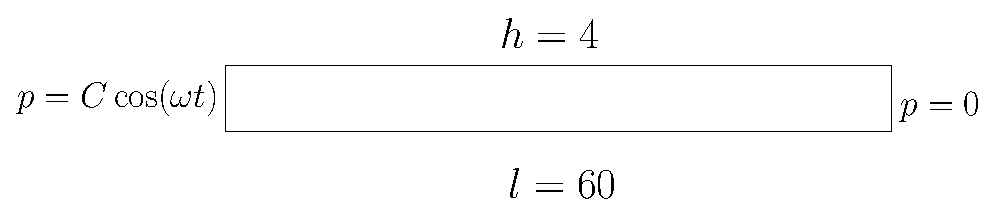
\includegraphics[width=\linewidth]{figures/Womersley}
\caption{Schematic of Womersley flow with dimensions as in the spinal cord}
\end{figure}
\end{center}

where C is a constant describing the strength of the pulse. Due to the assumption of axial flow only, the momentum equation in x-direction gives:
\begin{align}
\pdi{v_1}{t} = -\frac{1}{\rho}\pdi{p}{x_1} + \nu \pdi{^2v_1}{x_2^2} \label{NS_easy}
\end{align}
The presented solution did not correspond to the simulations at all, therefore an opportunity to utilize the symbolic python package sympy arised. The solution presented by Langlois and Deville was
\begin{align}
v_1 = -\frac{C}{\omega}\Bigg{[}\Big{(}1 - \frac{f_1(\omega,x_3)}{f_3(kh)}\Big{)}\sin(\omega t) - \frac{f_2(\omega,x_3)}{f_3(kh)}\cos(\omega t)\Bigg{]}
\end{align}
where
\begin{align}
k & = \sqrt{\frac{\omega}{2\nu}} \\
cc(x) & = \cos(x)\cosh(x) \\
ss(x) & = \sin(x)\sinh(x) \\
f_1(\omega,x_3) & = cc(kx_3)cc(kh) + ss(kx_3)ss(kh) \\
f_2(\omega,x_3) & = cc(kx_3)ss(kh) - ss(kx_3)cc(kh) \\
f_3(\omega) & = cc^2(\omega) + ss^2(\omega)
\end{align}
In sympy, even a complicated solution like this is easy to verify. The package lets the user define symbols to work with. Regular multiplication and general python functions can also be used. 
\begin{cverbatim}
from sympy import *
x3, C, x, h, t, w, nu = symbols('x3 C x h t w nu')
k = sqrt(w/(2*nu))
def cc(x):
	return cos(x)*cosh(x)
.
.
.

f3 = cc(w)**2 + ss(w)**2 

u = -C/w*((1-f1/f3)*sin(w*t) - f2/f3*cos(w*t))   # presented solution
d2u = nu*diff(diff(u,x3),x3)
dt = diff(u,t)

print simplify(d2u-dt)
\end{cverbatim}

From \eqref{NS_easy} the code snippet should print the pressure gradient divided by the density
\begin{align}
\frac{1}{\rho}\pdi{p}{x_3} = C\cos(\omega t)
\end{align}
This was not the case. Some error with the sign of the solution must have been made. 
\\
The solution
\begin{align}
v_1 = -\frac{C}{\omega}\Bigg{[}\Big{(}1 - \frac{f_1(\omega,x_3)}{f_3(kh)}\Big{)}\sin(\omega t) + \frac{f_2(\omega,x_3)}{f_3(kh)}\cos(\omega t)\Bigg{]} \label{Womersley}
\end{align}
Where the sign before the cos-term has been changed, yielded the correct pressure gradient, and hence this solution was used when error-estimates were investigated. 


\subsection{A penalty method for the boundary conditions}
To understand the problems arising with Neumann Conditions on both inlet and outlet we first consider the convection-diffusion equation. 
\begin{alignat}{3}
-\mu \nabla ^2 u + \mathbf{v}\cdot\nabla u & = f && \text{ in } \Omega \\
u & = u_0 && \text{ on } \partial \Omega_D \\
\mu \pdi{u}{n} & = g && \text{ on } \partial \Omega_N \label{ConvDiff}
\end{alignat}
Where $u$ is an unknown function, $\mathbf{v}$ is a prescribed velocity, $\mu$ is a diffusion constant and $f$ is a source term. The weak formulation reads:
\\
\\
\textit{Find } $u \in H^1_{u_0}$
\begin{align}
\mu (\nabla u, \nabla \phi)_\Omega+ (\mathbf{v} \cdot \nabla u, \phi)_\Omega = (f,\phi)_\Omega + (g,\phi)_{\partial \Omega_N} \text{ for all } \phi \in H^1_{0}.
\end{align}
Where the subscript on the two H-spaces indicate the values for functions on $\partial \Omega_D$ for these spaces. 
\\
\\
What has not been mentioned so far is the existence and uniqueness of the finite element solutions. To establish some concepts addressing these questions we let V denote a function space (in particular, V is a Hilbert space which has to satisfy given conditions on the associated inner product), and the inner product is denoted $(\cdot,\cdot)_V$ and the norm $||\cdot||_V$, (see e.g. Elman et al \cite{Elma14}) and define the following
\begin{definition}{(Coercivity)} \\
A bilinear form $a(\cdot,\cdot)$ is said to be \textit{coercive} with respect to the norm $||\cdot||_V$ if there is a positive constant $\gamma$ such that 
\[ a(u,u) \geq \gamma ||u||_V^2 \text{ for all } u \in V \]
\end{definition}
\begin{definition}{(Continuity)} \\
A bilinear form $a(\cdot,\cdot)$ is \textit{continuous} with respect to the norm $||\cdot||_V$ if there is a positive constant $\Gamma$ such that 
\[ a(u,u) \leq \Gamma ||u||_V||\phi||_V \text{ for all } u,\phi \in V \]

A linear functional L($\phi$) is \textit{continuous} with respect to $||\cdot||_V$ if there is a constant $\Lambda$ such that
\[ L(\phi) \leq \Gamma ||\phi||_V \text{ for all } \phi \in V \]
\end{definition}
In order to have a well posed problem, and ensure the existence of a unique solution $u \in V$ satisfying
\begin{align}
a(u,\phi) = L(\phi) \text{ for all } \phi \in V
\end{align}
 $a(\cdot,\cdot)$ and $L(\cdot)$ have to satisfy these criteria. This is commonly known as the Lax-Milgram lemma.\\
The convection term
\begin{align}
c(u,\phi) = (\mathbf{v}\cdot \nabla u, \phi)_\Omega \label{Conv}
\end{align}
makes this problem very different from the Poission-problem \eqref{Poisson},\eqref{Poisson_D}, \eqref{Poisson_N}, used when introducing the finite element method. 
In the light of the previous definitions we apply Green's theorem to \eqref{Conv}
\begin{align}
c(u,\phi) & = \int_\Omega \phi\mathbf{v} \cdot \nabla u \mathrm{d}x \\
& = - \int_\Omega u \mathbf{v} \cdot \nabla \phi  \mathrm{d}x - \int_\Omega u \phi \nabla \cdot \mathbf{v} \mathrm{d}x  + \int_{\partial \Omega_N} u \phi \mathbf{v} \cdot \mathbf{n} \mathrm{d}S \\
& = - c(\phi,u) + \int_{\partial \Omega_N} u \phi \mathbf{v} \cdot \mathbf{n} \mathrm{d}S
\end{align}

Where the last step follows from the assumption of incompressibility. From this
\begin{align}
c(u,u) = \frac{1}{2}\int_{\Omega_N} u^2 \mathbf{v} \cdot \mathbf{n} \mathrm{d}S
\end{align}
It is obvious that a Neumann condition on the inflow boundary, where $\mathbf{v}$ and $\mathbf{n}$ points in opposite directions, makes a negative contribution to the bilinear form $a(u,u)$. Therefore coercivity can not be completely ensured, and it typically depends on the magnitude of the velocity at the inlet. 
\\
\\
In several problems, prescribing Neumann conditions are simpler than providing inlet velocities. The pressure is set as a scalar value and can be assumed to have no spatial variation over the boundaries if the model has flat surfaces with normals aligned with the longitudional axis on the inlet and outlet. 
\\
\\
Barth and Carey \cite{Bart07} have described a penalty method for imposing the boundary conditions \eqref{P_out}. This was needed as horizontal flow at, and close to the boundaries caused problems interacting with the elastic spinal cord. The penalty method consists of adding a term at the relevant boundaries, penalizing parts where the boundary condition do not hold. For the velocity, we want $\mathbf{v} - (\mathbf{v}\cdot \mathbf{n})\mathbf{n}$ on the boundary, therefore the first variation of the least squares penalty functional is added to the original variational formulation
\begin{align}
I(\mathbf{v}) = \frac{1}{2\epsilon}\int_{\partial \Omega_p}\big{[}\mathbf{v} - (\mathbf{v}\cdot \mathbf{n})\mathbf{n}\big{]}\cdot\big{[}\mathbf{v} - (\mathbf{v}\cdot \mathbf{n})\mathbf{n}\big{]} \mathrm{d}s
\end{align}
where $0<\epsilon<<1$ is the penalty parameter. The contribution from the first variation will be
\begin{align}
I'(\mathbf{v})(\mathbf{\Phi}) = \frac{1}{\epsilon}\int_{\partial \Omega_p}\big{[}\mathbf{v} - (\mathbf{v}\cdot \mathbf{n})\mathbf{n}\big{]}\cdot\big{[}\mathbf{\Phi} - (\mathbf{\Phi}\cdot \mathbf{n})\mathbf{n}\big{]} \mathrm{d}s
\end{align}
This term will clearly contribute positively to the bilinear form and the penalty parameter should ensure that this contribution is large.
The method is tested on the coupled CFD solver, first with one time step of the Backwards Scheme and gradually refinement of the rectangular mesh. The time step is small, so the error introduced by the time discretization is negligible.
\begin{table}[!ht]
  \begin{center}
  \begin{tabular}{l | l | l | l | l | l}
    N & dofs &  $||v-v_h||_{L^2}$ & rate & $||v-v_h||_{H^1}$ & rate \\ \hline
     4 &    187 & 1.00e+00 & -- & 6.65e+00 & -- \\ \hline
     8 &    659 & 1.50e-01 & 2.739 & 1.95e+00 & 1.768 \\ \hline
    16 &   2467 & 1.91e-02 & 2.977 & 4.95e-01 & 1.981 \\ \hline
    32 &   9539 & 2.39e-03 & 2.997 & 1.24e-01 & 1.997 \\ \hline
    64 &  37507 & 2.99e-04 & 2.998 & 3.10e-02 & 1.999 \\ \hline
    \hline 
  \end{tabular}
  \caption{Errors P2-P1 elements}
  \end{center}
\end{table}


\begin{table}[!ht]
\begin{center}
  \begin{tabular}{l | l | l | l | l | l}

    N & dofs & $||v-v_h||_{L^2}$ & rate & $||v-v_h||_{H^1}$ & rate \\ \hline
     4 &    419 & 1.42e+01 & -- & 1.43e+02 & -- \\ \hline
     8 &   1539 & 7.84e-01 & 4.180 & 1.57e+01 & 3.186 \\ \hline
    16 &   5891 & 4.75e-02 & 4.045 & 1.90e+00 & 3.047 \\ \hline
    32 &  23043 & 2.97e-03 & 3.999 & 2.38e-01 & 3.000 \\ \hline
    64 &  91139 & 1.86e-04 & 3.999 & 2.97e-02 & 2.999 \\ \hline
    \hline
  \end{tabular}
  \end{center}
  \caption{Errors P3-P2 elements}
\end{table}


C = 1000 \\
dt = 0.001 \\
T = 0.1 \\
Backward Euler 1st order \\
\begin{figure}[!ht]
\begin{center}
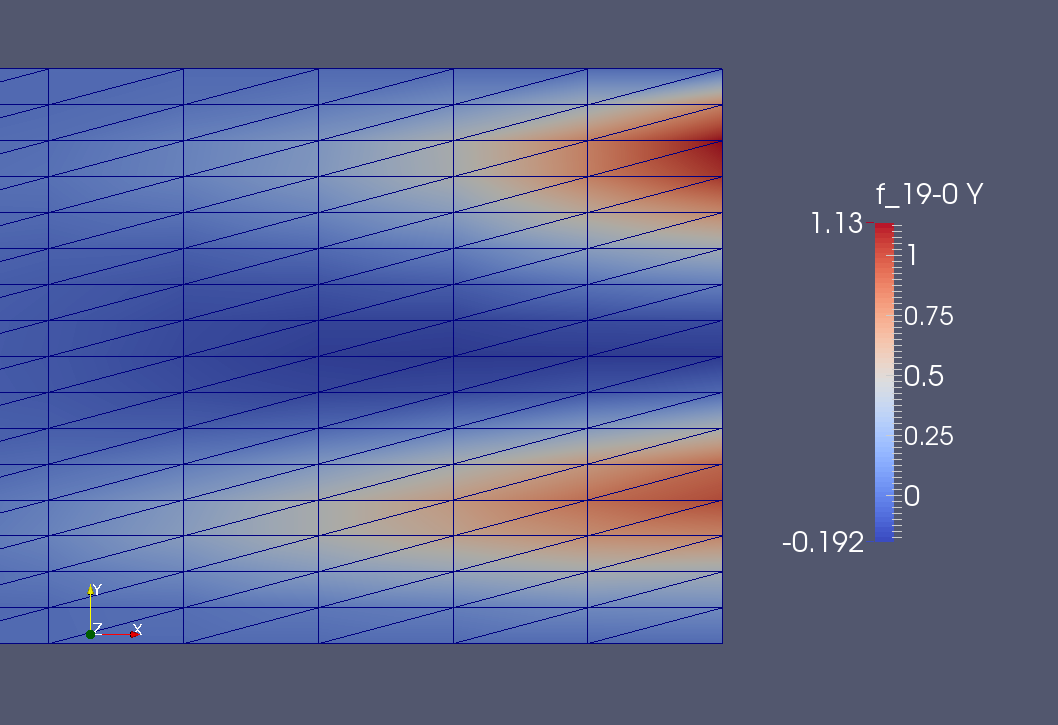
\includegraphics[width=0.48\linewidth]{figures/Womersley_no_penalty_BE_01}\hspace{0.04\linewidth}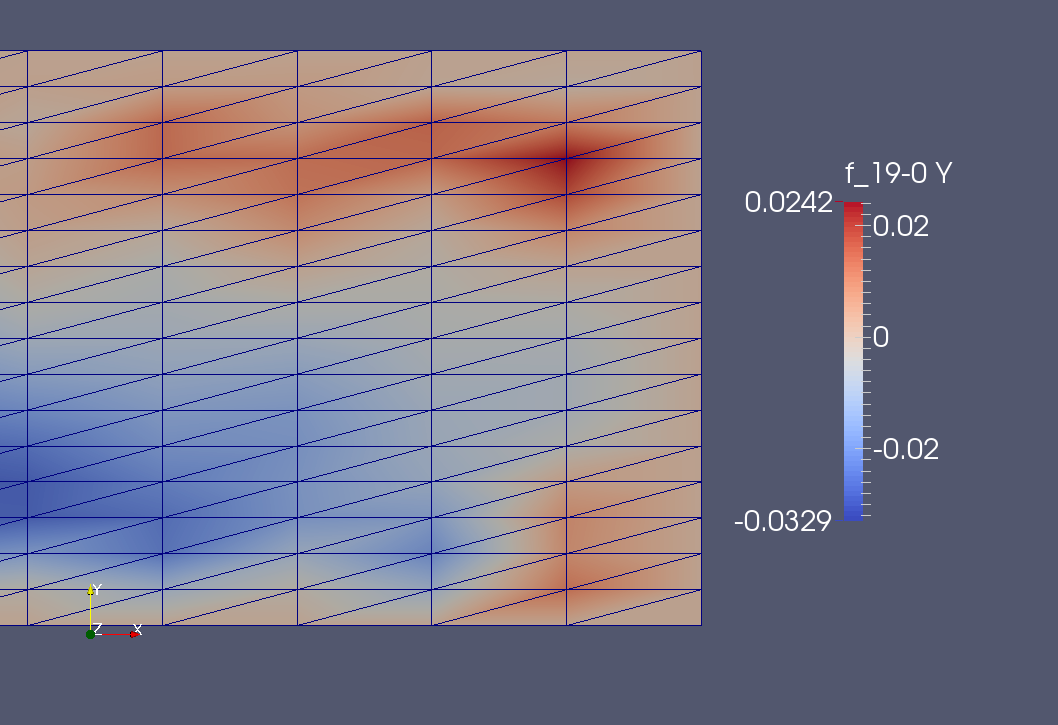
\includegraphics[width=0.48\linewidth]{figures/Womersley_penalty_BE_01}
\caption{Velocity distribution in y-direction at t=0.1 without (left) and with the penalty method at the outlet. These velocities are of several orders lower than in the x-direction, but accumulates over time without the penalty method}
\end{center}
\end{figure}


